% This is LLNCS.DEM the demonstration file of
% the LaTeX macro package from Springer-Verlag
% for Lecture Notes in Computer Science,
% version 2.4 for LaTeX2e as of 16. April 2010
%
\documentclass{llncs}
%
\usepackage{makeidx}  % allows for indexgeneration
% For figures
\usepackage{graphicx} % more modern
%\usepackage{epsfig} % less modern

\usepackage{subcaption}
\usepackage{color}
%\usepackage{subfig}%[caption=false,font=footnotesize]

% For citations
\usepackage{natbib}

% For algorithms
\usepackage{algorithm}
\usepackage{algorithmic}
\usepackage{amsmath}
% As of 2011, we use the hyperref package to produce hyperlinks in the
% resulting PDF.  If this breaks your system, please commend out the
% following usepackage line and replace \usepackage{icml2012} with
% \usepackage[nohyperref]{icml2012} above.
\usepackage{hyperref}

% Packages hyperref and algorithmic misbehave sometimes.  We can fix
% this with the following command.
\newcommand{\theHalgorithm}{\arabic{algorithm}}

%-------------------------------------------------------------
%                      Own Commands
%-------------------------------------------------------------
\usepackage{amsmath}
\newcommand{\cbn}{\textsc{Cbn}}
\newcommand{\bn}{\textsc{Bn}}
\newcommand{\huang}[1]{\textcolor{blue}{#1}}
\newcommand{\mycomment}[1]{\textcolor{red}{( ...#1 )}}
\renewcommand{\algorithmiccomment}[1]{/* #1 */}
\def\ci{\perp\!\!\!\perp}
\def\dep{\perp\!\!\!\perp\!\!\!\!\!\!\!/\,\,\,\,}
% Theorem & Co environments and counters
%\newtheorem{theorem}{Theorem}[section]
%\newtheorem{lemma}[theorem]{Lemma}
%\newtheorem{corollary}[theorem]{Corollary}
%\newtheorem{remark}[theorem]{Remark}
%\newtheorem{definition}[theorem]{Definition}
\newtheorem{equat}[theorem]{Equation}
%\newtheorem{example}[theorem]{Example}
%-------------------------------------------------------------

\begin{document}
%
\frontmatter          % for the preliminaries
%
%\pagestyle{headings}  % switches on printing of running heads
%\addtocmark{Hamiltonian Mechanics} % additional mark in the TOC
%%
%\tableofcontents
%
\mainmatter              % start of the contributions
%
\title{ Low-Budget Learning from Multiple Experts}
%
%\titlerunning{Hamiltonian Mechanics}  % abbreviated title (for running head)
%                                     also used for the TOC unless
%                                     \toctitle is used
%
\author{Bojan  Kolosnjaji\inst{1} \and Huang Xiao\inst{2} 
	\and Claudia Eckert\inst{1}\inst{2} }
%Jeffrey Dean \and David Grove \and Craig Chambers \and Kim~B.~Bruce \and
%Elsa Bertino}
%
\authorrunning{Bojan Kolosnjaji et al.} % abbreviated author list (for running head)
%
%%%% list of authors for the TOC (use if author list has to be modified)
%\tocauthor{Ivar Ekeland, Roger Temam, Jeffrey Dean, David Grove,
%Craig Chambers, Kim B. Bruce, and Elisa Bertino}
%
\institute{Technical University of Munich, Fraunhofer AISEC\\
\email{kolosnjaji@sec.in.tum.de, huang.xiao@aisec.fraunhofer.de, eckert@sec.in.tum.de}
%\\ WWW home page:
%\texttt{https://www.aisec.fraunhofer.de/}
%\and
%Universit\'{e} de Paris-Sud,
%Laboratoire d'Analyse Num\'{e}rique, B\^{a}timent 425,\\
%F-91405 Orsay Cedex, France
}

\maketitle              % typeset the title of the contribution

\begin{abstract}
Learning from multiple sources of labeled data can increase the confidence of a machine learning system if the expertise of different labelers can be assembled efficiently. However, using a large amount of labelers in the test time can be expensive in the long run. For instance, in crowdsourcing, we have to pay each labeler in order to get the annotations. In Internet-of-Things, obtaining data from multiple sensors for direct fusion incurs high communication overhead. 

In this paper, we propose a method for training a classification system from data labeled by multiple client annotators, where only a small subset of annotators are optimally chosen to reduce communication effort. 
We define an iterative optimization procedure where the sparsity of a client weight vector is enforced while reducing the overall classification error. Using a set of experiments with real and synthetic data, we show that our approach can pertain the classification performance as on the complete set of labelers while reducing the communication effort by over 70\% on several different tasks.

\keywords{machine learning, communication-efficiency, crowdsourcing, Internet-of-Things}
\end{abstract}
%

\section{Introduction}
Supervised machine learning depends on our ability to gather a large set of labeled data. In a high number of scenarios, we can benefit from labeled data gathered by querying multiple separate sources with varying reliability and join this data into one machine learning model. However, many times we are limited in the number of data sources that we are allowed to use, because of budget constraints, limited processing power or insufficient communication bandwidth. This causes the need for a framework that would enable resource-efficient combination of labeled data from multiple sources.

First important fitting scenario to this framework is crowdsourcing. When using crowdsourcing systems such as Amazon Mechanical Turk, we can gather labelled data from multiple annotators. After gathering this training data, we need to join the labelling decisions and train one machine learning system while leveraging all of the annotations. Relying on a concept of \textit{wisdom of crowds}, we can assume that if we gather data from a sufficient number of people, on average most of them will give correct labelling decision. However, gathering data from a large amount of annotators can be expensive, as workers on Amazon Mechanical Turk require payment for their work. Therefore we would benefit from a procedure of prior determination of the annotators' expertise. In this case, the joining process can be optimized by estimating the expertise of the annotators, selecting the optimal subset and determining weights of the annotators' labels. Moreover, in a rising area of \textit{Internet of Things} (IoT) we can have similar problems. In IoT systems, a large number of sensors provide information about the environment. Communication among multiple sensors can be costly in terms of processing power. Furthermore, this communication can be done among sensors that are limited with power consumption constraints. Furthermore, in intrusion detection it is useful to use results from multiple anomaly detection systems. For example, although there are multiple antivirus programs that can label software as benign or malicious programs of certain type, only a minority of the programs contain updated labels for newest malware families and classify malware with high granularity. Therefore it would be useful to find a subset of label sources that are reliable enough to be used for malware triage purposes.

There are multiple papers that deal with estimating the expertise of labelers when using \textit{wisdom of crowds}. For example, Welinder et al. \cite{welinder2010multidimensional} determine groups of annotators with similar expertise, and find particular phenomena such as "schools of thought" and specialist experts in certain types of image labeling tasks. Tian and Zhu~\cite{tian2012learning} investigate the annotator behavior in executing more complex labeling tasks, such as answering if an image is beautiful or if it contains a car. Zhang et al.~\cite{zhang2013learning} propose a method to filter out novice labelers. However, their method is specific to Gaussian Mixture Models. Rodrigues et al.~\cite{rodrigues2014gaussian} determine a similar procedure specific to Gaussian Processes. Bi et al.~\cite{bi2014learning} argue that the factors that determine the annotators' labeling performance, apart from the expertise, can also be the worker's dedication to the task, his/her default labeling judgement and sample difficulty. However, they do not go further in determining the optimal subset of annotators. On the other hand, Li and Liu~\cite{li_liu_2015} propose a combinatiorial procedure to find this optimal subset. However, such combinatorial procedures are very resource-intensive, especially for a large initial set of annotators.

On the other hand, there are are also multiple more theoretical frameworks. For example, Wang et al.~\cite{wang2015efficient} propose a selection of sensors based on Directed Acyclic Graphs (DAGs) in resource-constrained scenarios. However, they do not deal with annotating data, so their ideas do not completely fit to our problem. 

We design a methodology that both selects an optimal subset of annotators from a set of training data and automatically determines the weights of the selected annotators. By forcing sparsity on our annotator weight vector during optimization, we get an accurate classification system that works well even with annotations from a small set of highly competent annotators. This gives us a low-budget supervised learning strategy, which is not specific to any particular learning algorithm.

In summary, we make the following contributions:
\begin{itemize}
\item We propose a methodology for selecting an optimal subset of workers in a classification system with multiple labelers
\item We create a procedure for selecting and determining weights of labelers independent of the type of machine learning methods selected for modeling the annotating process
\item Using a set of experiments with both real and synthetic data, we show that we can obtain an accurate classification system with the optimized annotator subset.
\end{itemize}  


\section{Methodology}

Our methodology is based on the scenario drawn on the \autoref{fig:scheme}. This scheme shows a common situation when a server acquires labels from multiple annotators. 

\begin{figure}
  \caption{Label aggregation scheme}
  \centering
    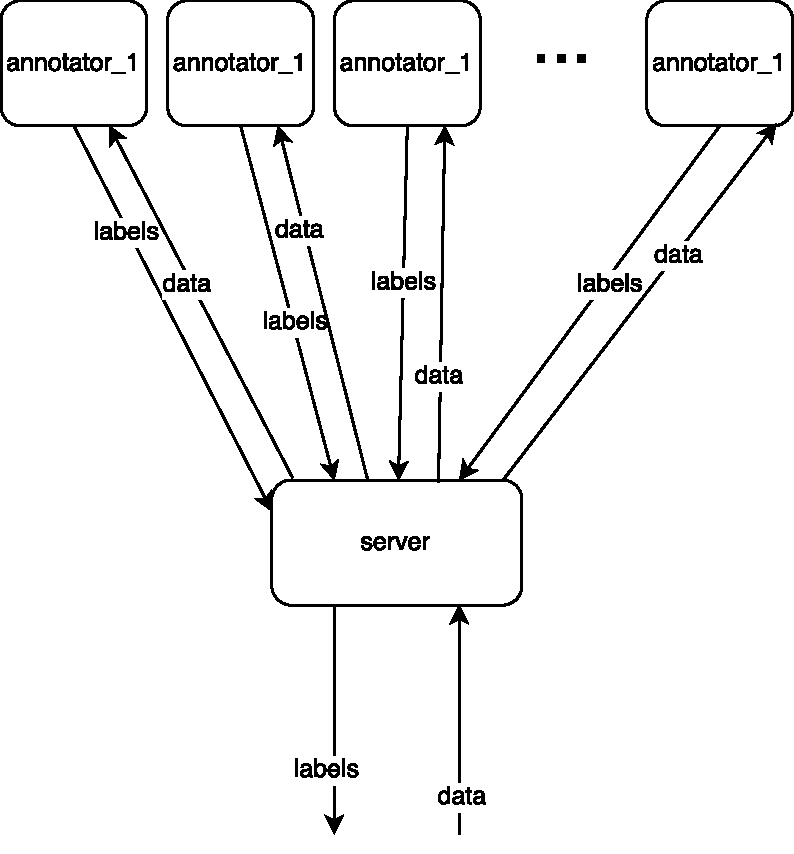
\includegraphics[width=0.5\textwidth]{figures/lowbudget.pdf}
  \label{fig:scheme}
\end{figure}

In training time, server forwards the training inputs to all the annotators in order to retrieve labels. Using the data labeled from a large set of annotators, the server trains a machine learning model that jointly learns the expertise of all the clients while minimizing the quadratic loss with respect to the ground truth.  

We design a method that would enable us to manage the tradeoff between model accuracy and communication effort. Furthermore, we impose a requirement that our methodology needs to be simple and compatible with a wide range of machine learning methods. 

Based on these requirements, our optimization model has a cost function consisting of three parts:

\begin{enumerate}
\item minimizing the cost with respect to the ground truth labels on the training set
\item minimizing the cost with respect ot the client annotations
\item making the client weight vector sparse (select a small subset of clients)
\end{enumerate}

The cost function for cross-entropy loss on ground truth, used in all our experiments, looks like the following:

\begin{equation}
\begin{split}
 L(w,v)= -\frac{1}{N} \sum_{n=1}^N (\hat{y}_n \log \sum_{i=1}^M v_i y_{ni} + (1-\hat{y}_n) \log(1-\sum_{i=1}^M v_i y_{ni})) + \\ + \psi \sum_{i=1}^{M} (y_{ni} - z_{ni})^2+\lambda \mid v \mid
\end{split} 
\end{equation}
subject to:
\begin{equation}
 \sum_{i=1}^{M} v_i = 1 
\end{equation}

\noindent where $ \hat{y}_n $ are ground truth labels for all training samples, $ y_{ni} $ are labels retrieved by querying  current client models, $z_{ni}$ are training labels from annotator clients, $v_i$ is a normalized vector of weights for all the clients. The final loss function consists of a crossentropy calculation for the empirical loss with respect to the ground truth, the quadratic loss with respect to the client annotations weighted by a parameter $\phi$ and the $L_1$-norm of the parameter vector $v$ weighted by another parameter $\lambda$.

We want to use $L_1$ regularization to minimize the client weight vector. This is similar to the \textit{Lasso} feature selection, except that we select clients instead of features. 

The gradient is defined with the following equations:
\begin{equation}
\begin{split}
 \frac{\partial L}{\partial w_j} = -\frac{1}{N} \sum_{n=1}^N (y_n \frac{1}{\sum_{i=1}^M v_i \hat{y}_{ni}} v_j \frac{\partial y_n}{\partial w_j} + (1-y_n) \frac{1}{1-\sum_{i=1}^M } v_j \frac{\partial y_n}{\partial w_j} + \\  \psi \sum_{i=1}^M 2 (y_{ni} - z_{ni} \frac{\partial y_n}{\partial w_j}  ))
\end{split}
\end{equation}

\begin{equation} \frac{\partial L}{\partial v_i} =  -\frac{1}{N} \sum_{n=1}^N (y_n \frac{1}{\sum_{i=1}^M v_i y_{ni}} + (1-\hat{y_n}) \frac{1} {1-\sum_{i=1}^M v_i y_{ni}} (-y_n) 
\end{equation}
The expression for the gradient $ \frac{\partial y_n}{\partial w_j}$ depends on the concrete method used to model the annotators.

For logistic regression we directly define the cost for the errors with respect to ground truth as crossentropy. However, with minimal changes our framework can also be usable with other machine learning methods. For example, we tested our methodology with neural networks as well, using a perceptron with one hidden layer. These methods, however, need to be convex or have a convex relaxation in order to still make a gradient-based optimization procedure work well.

In order to still use gradient descent as a convex optimization method with the $L_1$ norm, we use iterative soft-thresholding~\cite{bredies2007iterative}, a type of generalized gradient descent optimization when updating the value of $v$. The update that we derived is the following:

\begin{equation}
 v= v + S_{\lambda} (v-t_s \frac{\partial L}{\partial v}, \lambda)
\end{equation}
where
\begin{equation}
S_{\lambda} (k, \lambda) = 
\left\{
	\begin{array}{ll}
		k-\lambda  & \mbox{if } k > \lambda  \\
		k+\lambda & \mbox{if } k < -\lambda \\
		0 & \mbox{otherwise}
	\end{array}
\right.
\end{equation}

Furthermore, we normalize the values in the vector $v$ in order to retrieve the proper values of client weights:

\begin{equation}
v = \frac{v}{\sum_{i=1}^M v_i}
\end{equation}

In case of multiclass classification, we define the loss function in a slightly different way, to accomodate with the fact that we need a label vector instead of scalar value:

\begin{equation}
 L(w,v)= -\frac{1}{N} \sum_{n=1}^N \sum_{k=1}^K (\hat{y}_{nk} \log \sum_{i=1}^M v_i y_{nik}) + \psi \sum_{i=1}^{M} (y_{ni} - z_{ni})^2+\lambda \mid v \mid
\end{equation}, 

subject to
\begin{equation}
 \sum_{i=1}^{M} v_i = 1 
\end{equation}

This time, $\hat{y}$ is a matrix and $y$ is a three-dimensional tensor. The optimization is done in a similar way, using projected gradient descent. We minimize the cross-entropy w.r.t the ground truth, as well as the squared difference of ground truth and annotator decision, while keeping the annotator vector sparse.

%Full expertise model:
%
%
%\begin{equation}
%\begin{split}
% L(w,v)= -\frac{1}{N} \sum_{n=1}^N (\hat{y}_n \log \sum_{i=1}^M v_{ni} y_{ni} + (1-\hat{y}_n) \log(1-\sum_{i=1}^M v_{ni} y_{ni})) + \\ \psi \sum_{i=1}^{M} (y_{ni} - z_{ni})^2+\sum_{n=1}^{N}\lambda \mid v_n \mid
%\end{split} 
%\end{equation}

\section{Results}

We use two datasets to evaluate our methodology of combining the expertise of different annotators. Furthermore, we test our approach using two different models of annotators: logistic regression model and a neural network model (perceptron with one hidden layer).

\subsection{Datasets}
In order to evaluate our approach, we use one dataset with real-life labelers and one with synthetic labelers. 

\subsubsection{Real-Life Labelers}
We obtained a real-life labeler set from the authors of a related paper about learning to predict from crowdsourced data by Bi et al.~\cite{bi2014learning}. This dataset consists of results from an experiment with 21 workers at the \textit{Amazon Mechanical Turk}. These workers executed 10 tasks, all of the tasks being binary classification of images. Since each worker has different expertise, the challenge is to determine the subset of highly competent workers and combine their abilities for a superior classification system.

\subsubsection{Synthetic Labelers}
In order to further examine the performance of our method, we also use a semi-synthetic data based on the well-known MNIST dataset~\cite{lecun1998mnist} for digit recognition with around 70000 images of digits. We use images from this data without change and we take labels for images as ground truth. However, we synthetically create annotators by training multiple classifiers with random 0.5\% of images from the original set. This gives us annotators that have expertise in labeling only a subset of images, that on average have 81\% accuracy on a holdout test set. We use this set of annotators to test if we can surpass the performance of a single particular annotator by combining a minority of them.

\subsection{Optimization process}

Furthermore, we look at how the value of the loss function changes while the optimization is running. We plot the loss against the number of iteration, which shows the steep decline of the loss value. This shows that using our gradient-based procedure we can get fast to a very accurate classification system. The graph is shown on \autoref{fig:optimization}.

Next, we execute a similar test with the parameter $v$. We look at how the number of nonzero elements of $v$ changes while optimization is running. In other words, we examine how the optimizer selects the competent annotators.

\begin{figure}[!htb]	
    \centering
    
    \begin{subfigure}[b]{0.45\textwidth}
        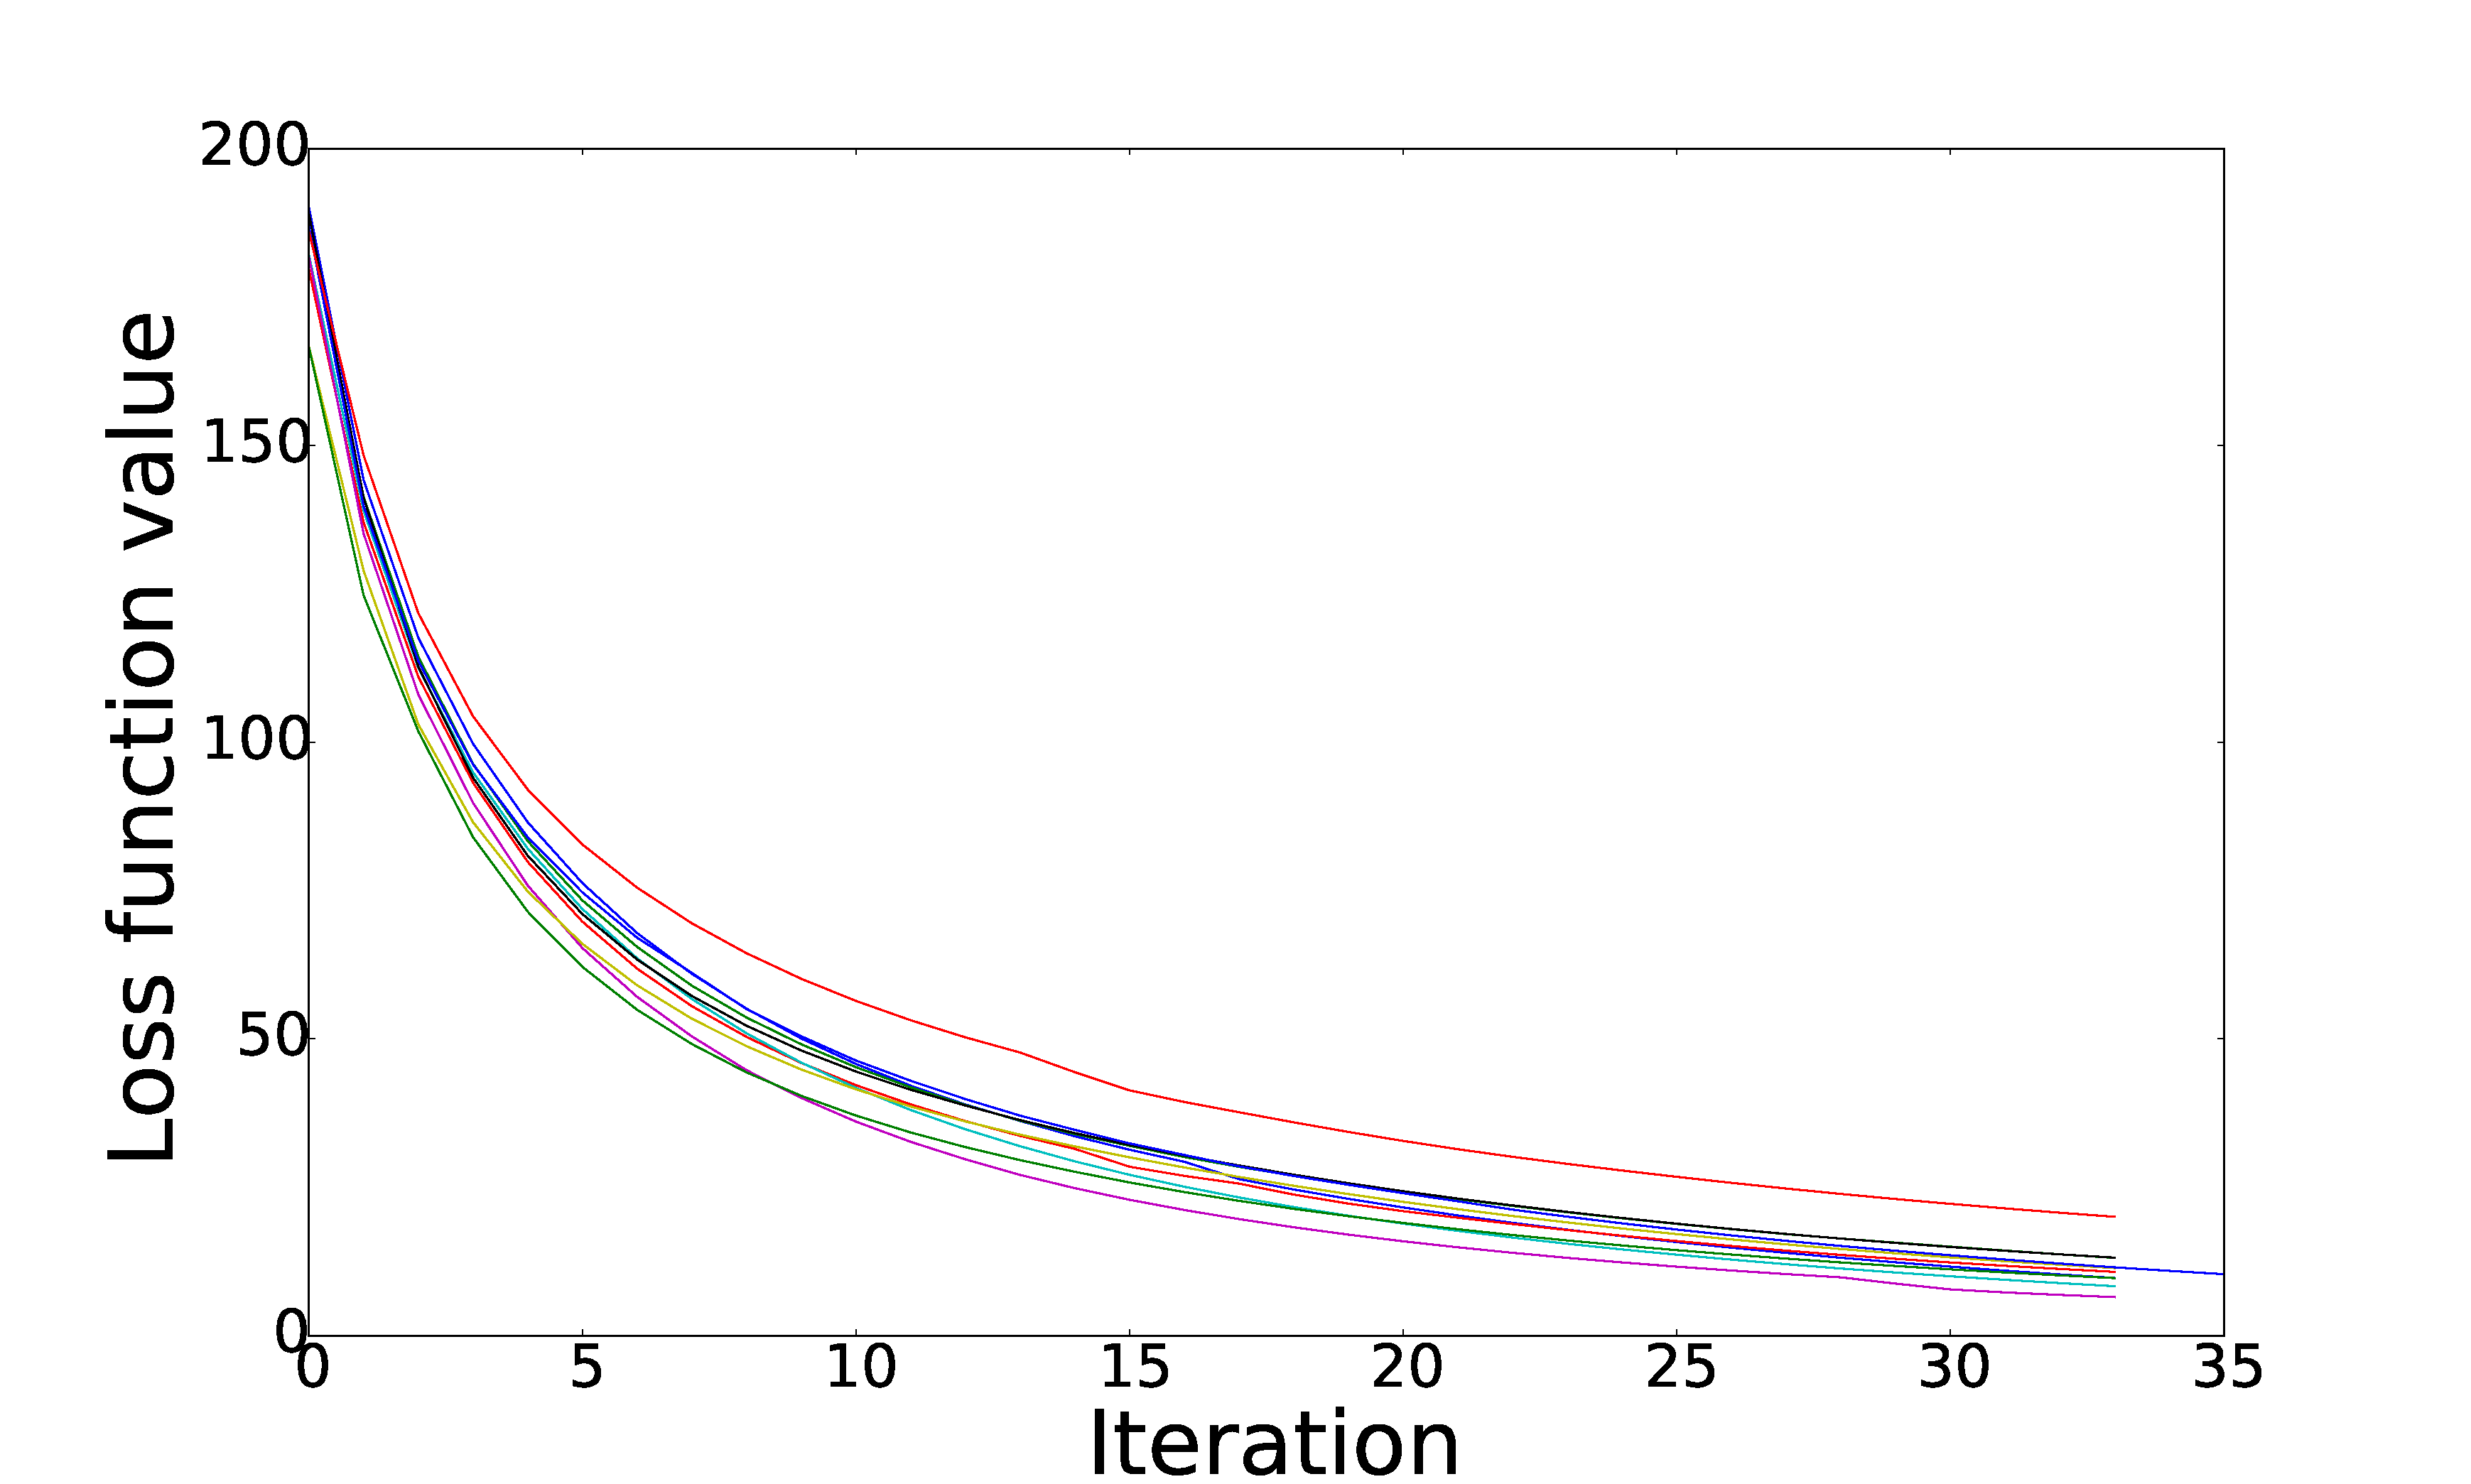
\includegraphics[width=\textwidth]{figures/loss_iteration_logreg}
        \caption{Loss minimization}

    \end{subfigure}
    \begin{subfigure}[b]{0.45\textwidth}
        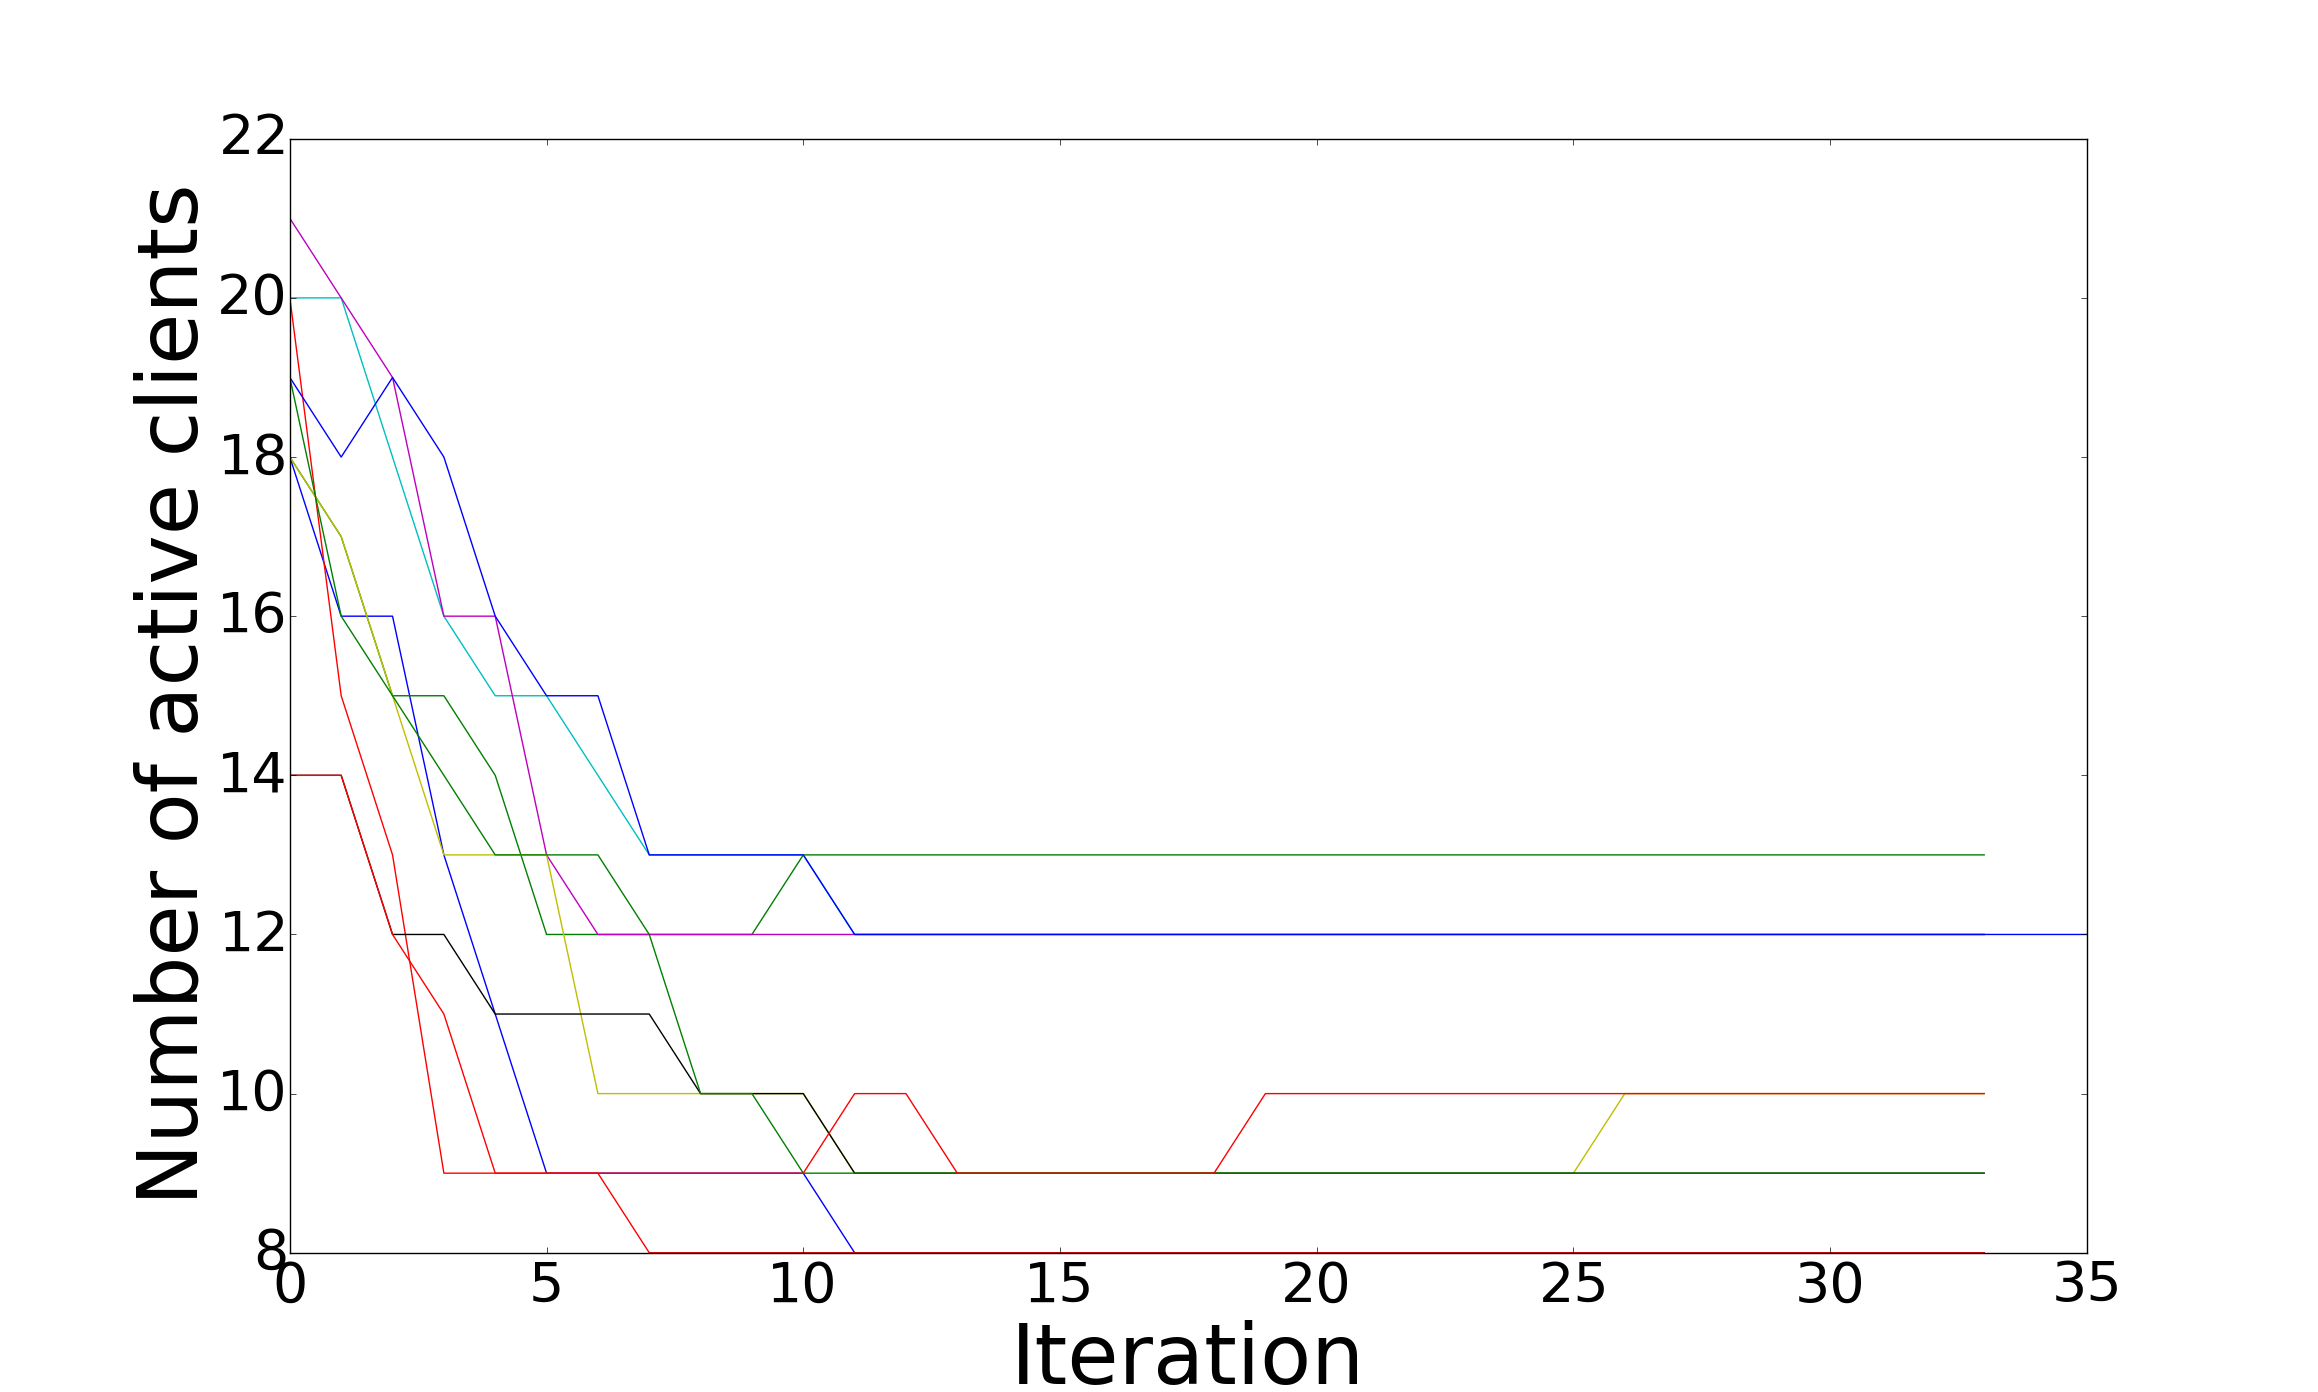
\includegraphics[width=\textwidth]{figures/v_iteration_logreg}
        \caption{Reduction of annotator subset}

    \end{subfigure}
    \caption{Training process}
    \label{fig:optimization}
\end{figure}

\subsection{Performance per task}

In the following figures we examine the breakdown of classification error rate per labeling task. We can notice on \autoref{fig:pertask} that the performance of our classifier ensemble has a high variation, both when using a neural network and logistic regression.

\begin{figure}[!htb]

    \centering
    \begin{subfigure}[b]{0.45\textwidth}
        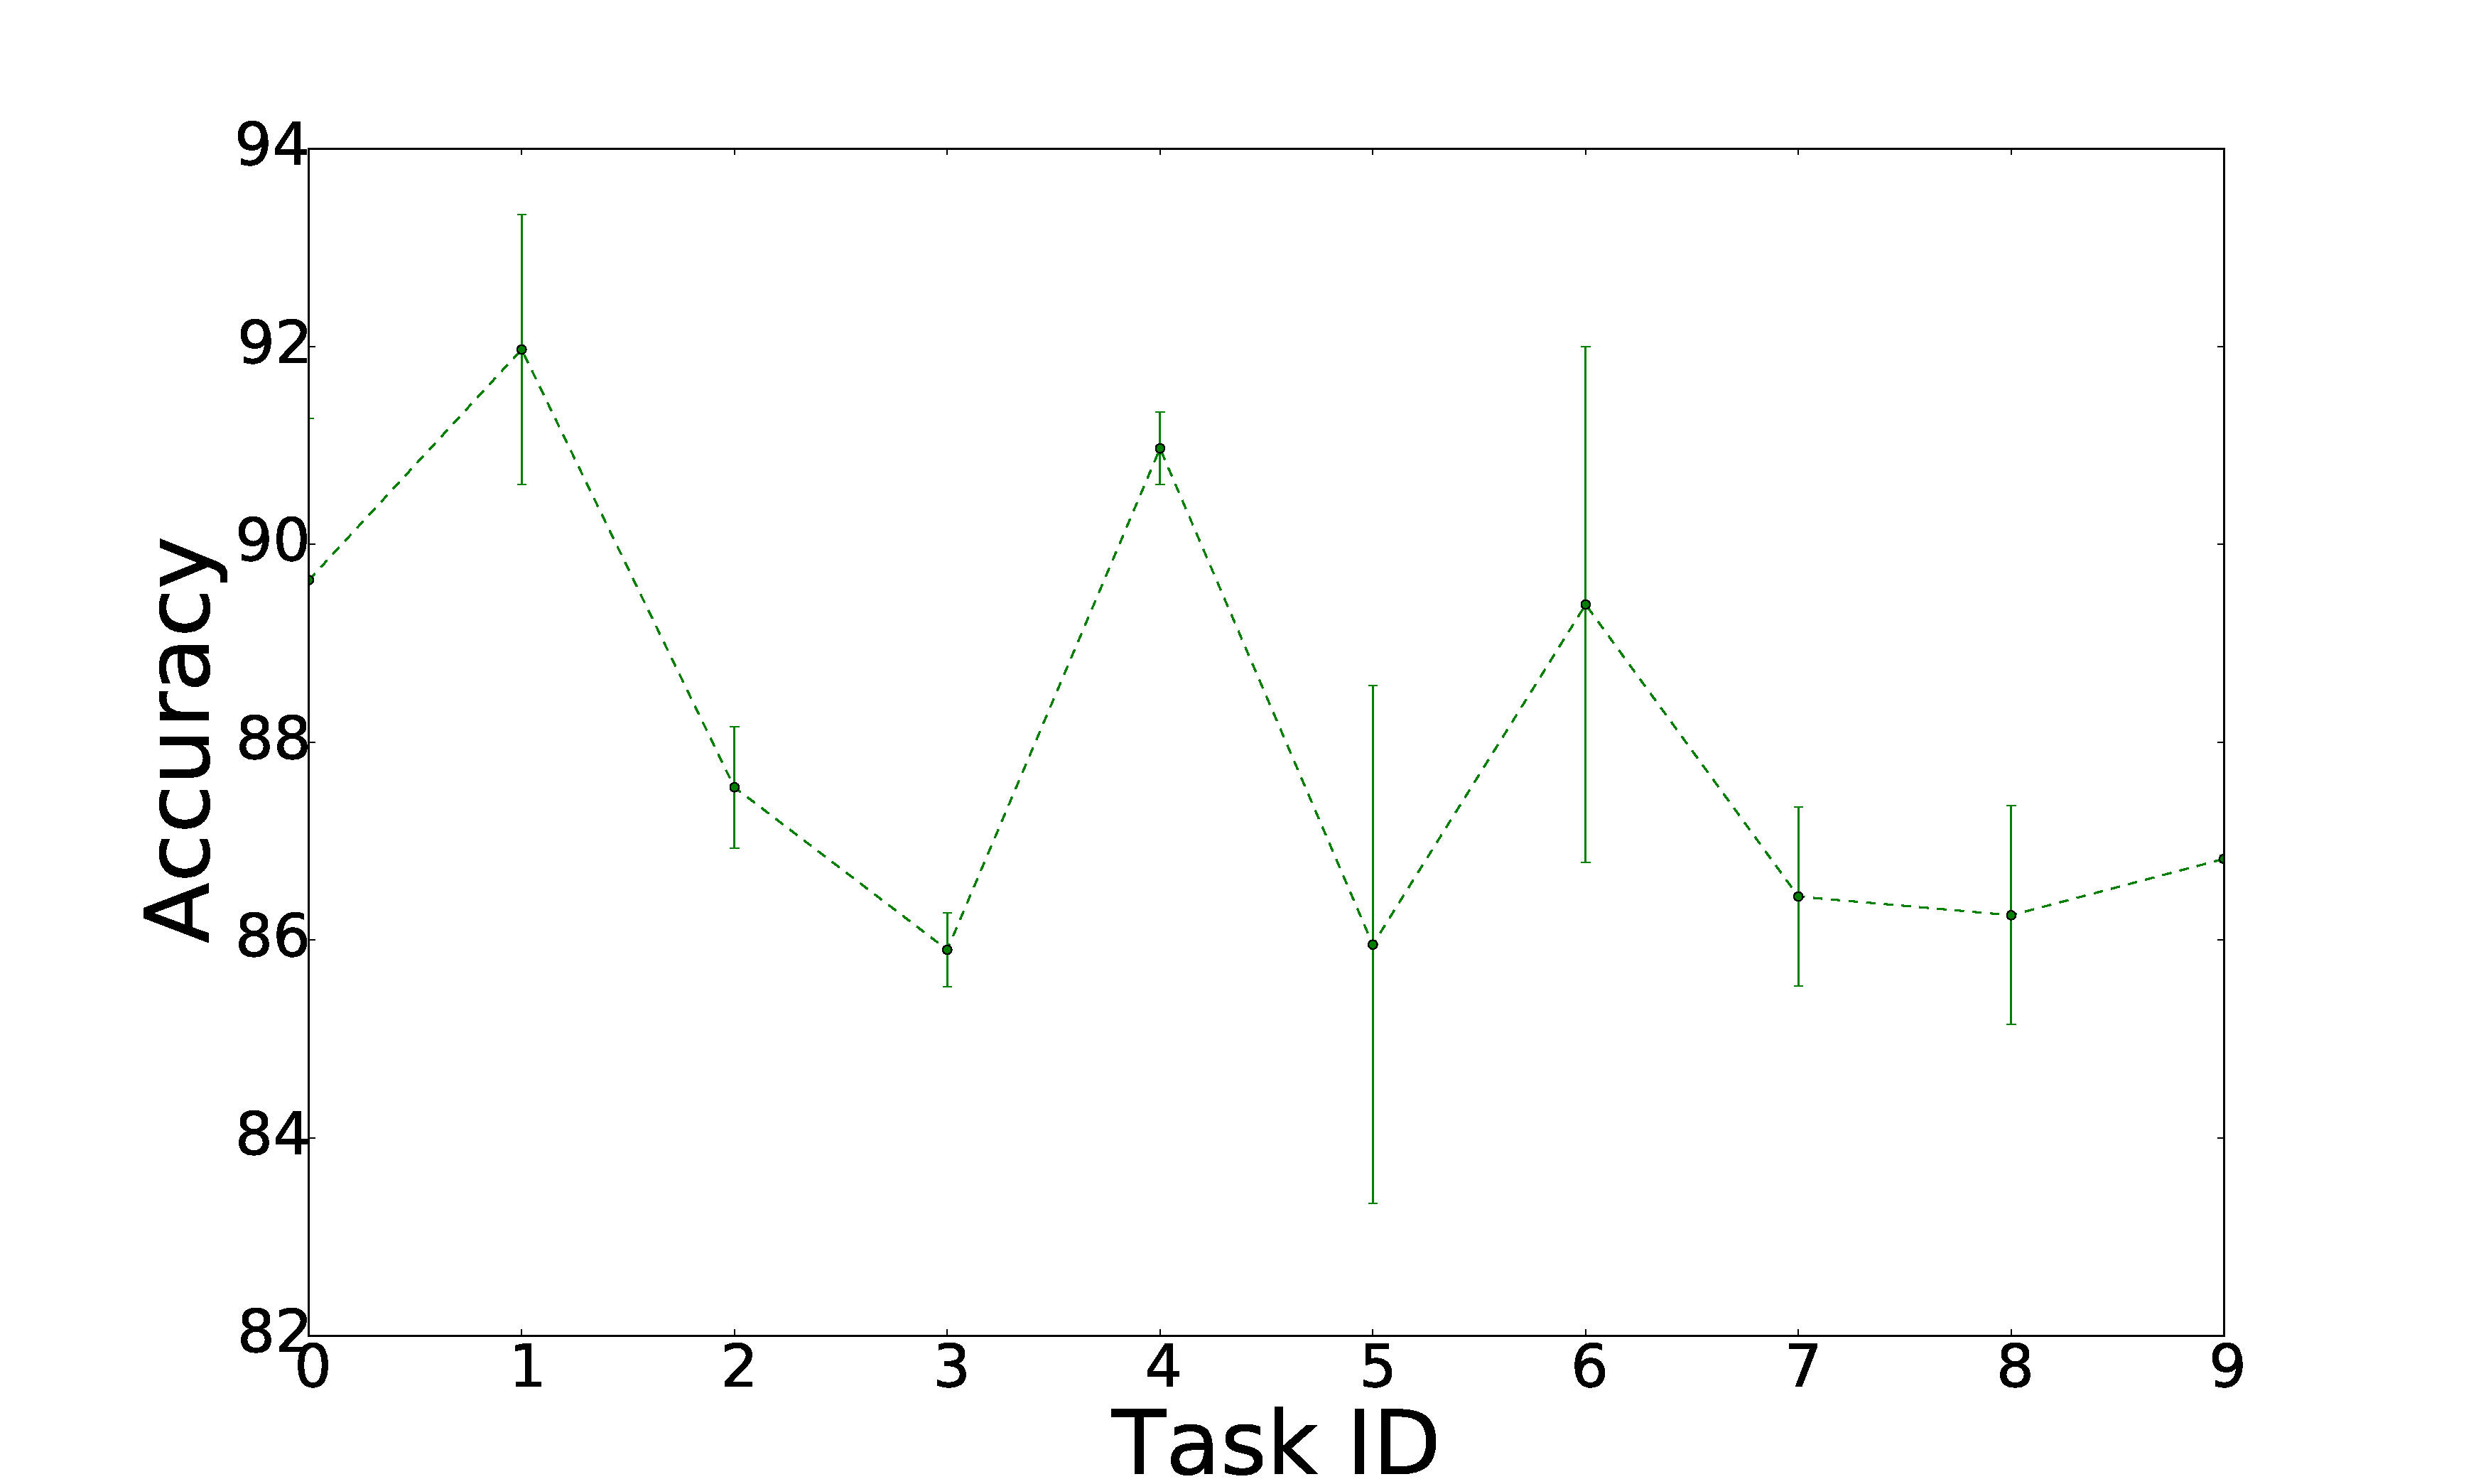
\includegraphics[width=\textwidth]{figures/task_logreg}
        \caption{Logistic regression}
    \end{subfigure}
    \begin{subfigure}[b]{0.45\textwidth}
        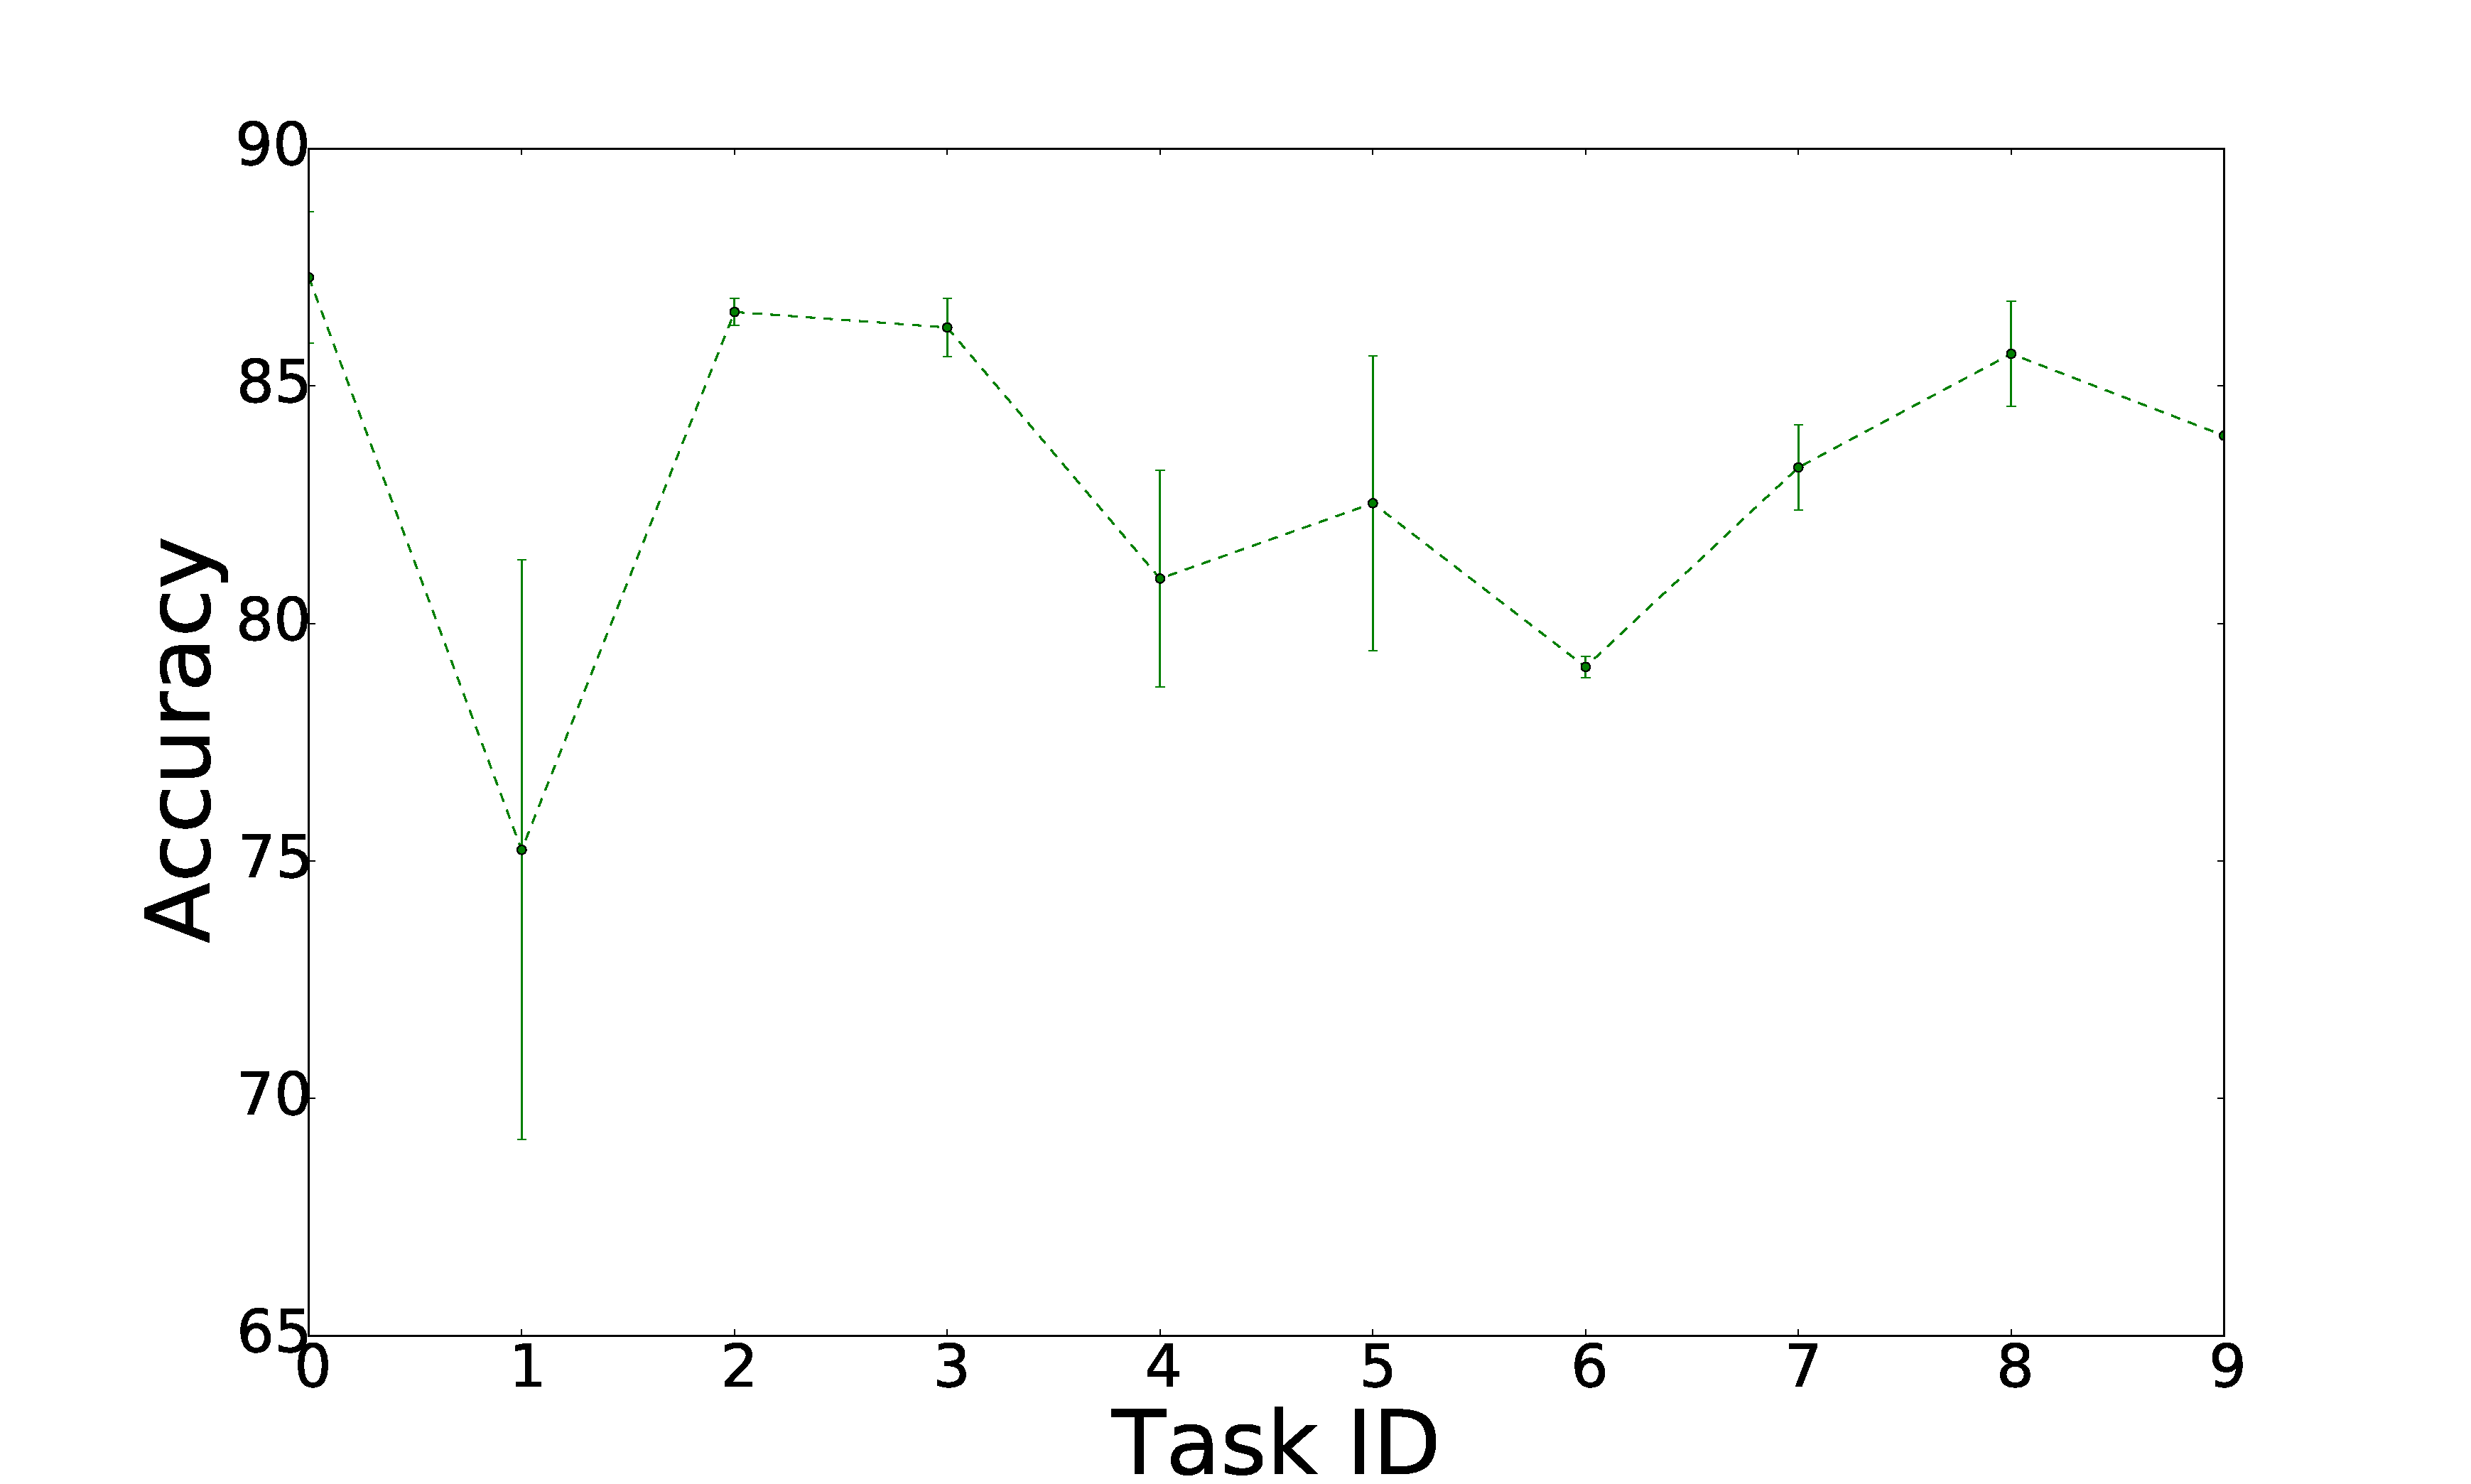
\includegraphics[width=\textwidth]{figures/task_mlp}
        \caption{Neural network}
    \end{subfigure}
    \caption{Performance per task}
    \label{fig:pertask}
    
\end{figure}


\subsection{Comparison with baseline ensemble methods}

Furthermore, we compare the performance of our scheme with annotator selection to some baseline ensemble methods, such as averaging annotator values and taking a majority vote. %Moreover, we also compare our performance with a system that randomly chooses annotators. 
This comparison is shown on Figure~\ref{fig:baseline}.

\begin{figure}[!htb]
    \centering
    \begin{subfigure}[b]{0.45\textwidth}
        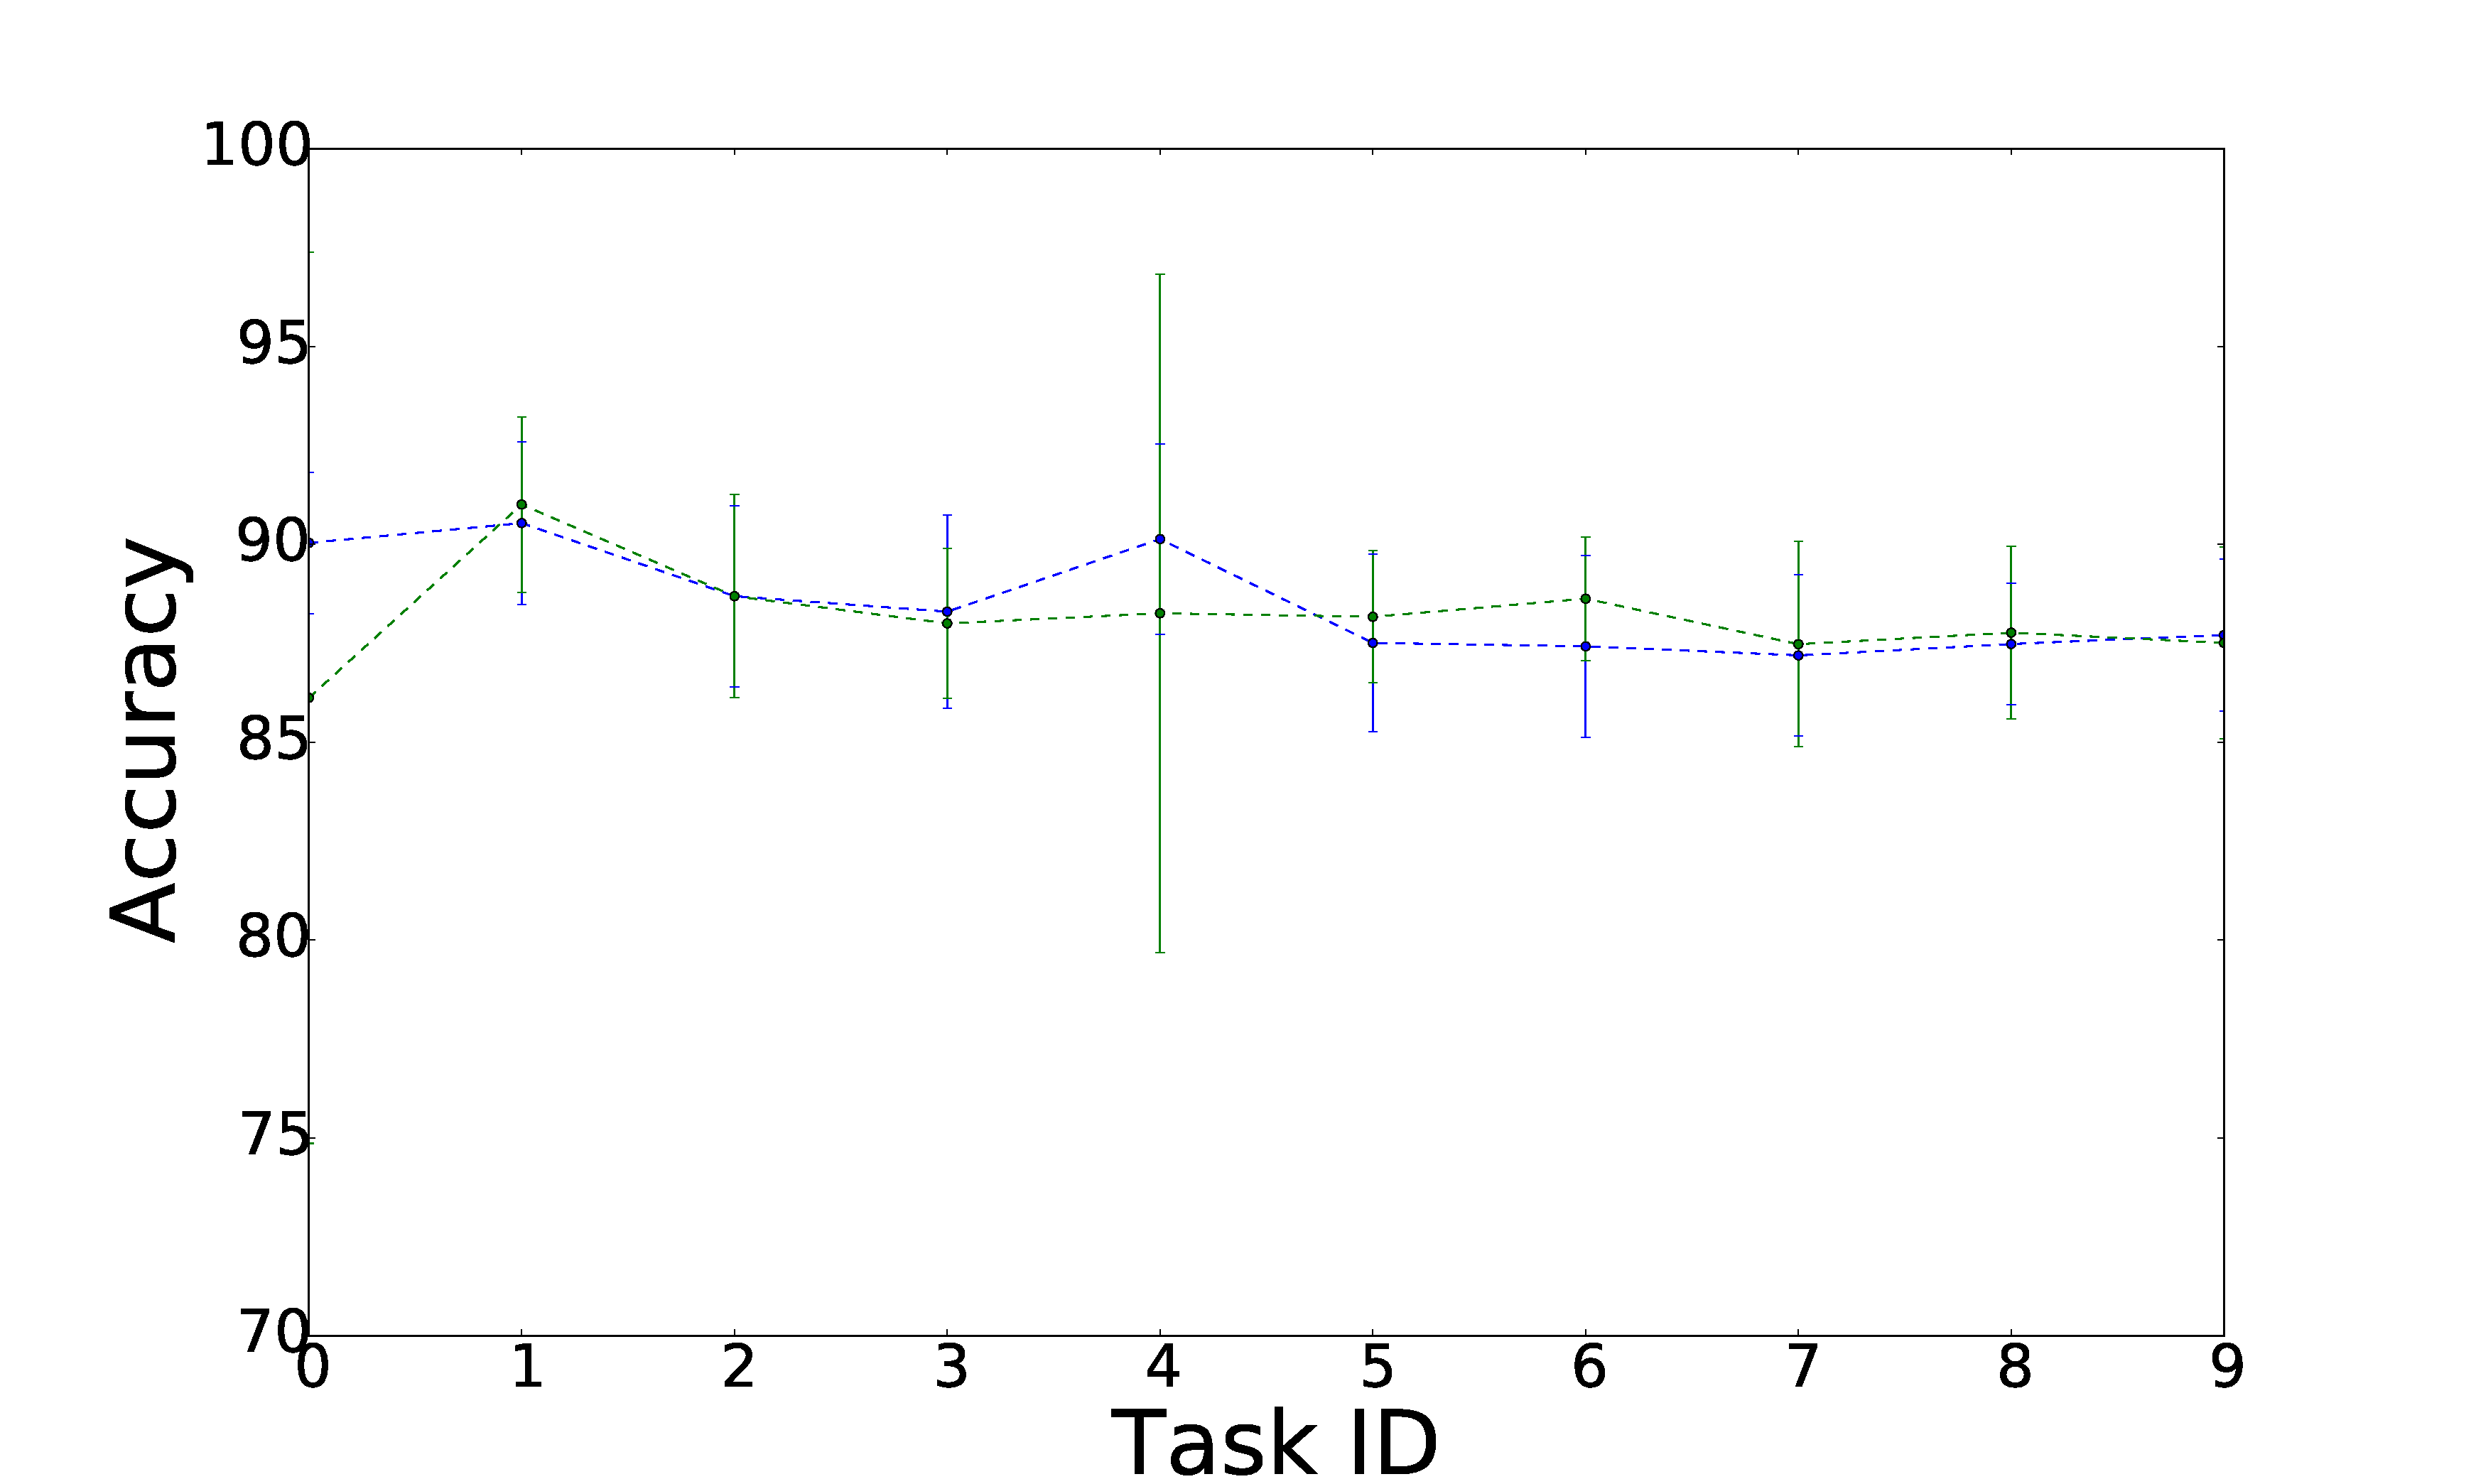
\includegraphics[width=\textwidth]{figures/comp_average}
        \caption{Logistic regression}
    \end{subfigure}
    \begin{subfigure}[b]{0.45\textwidth}
        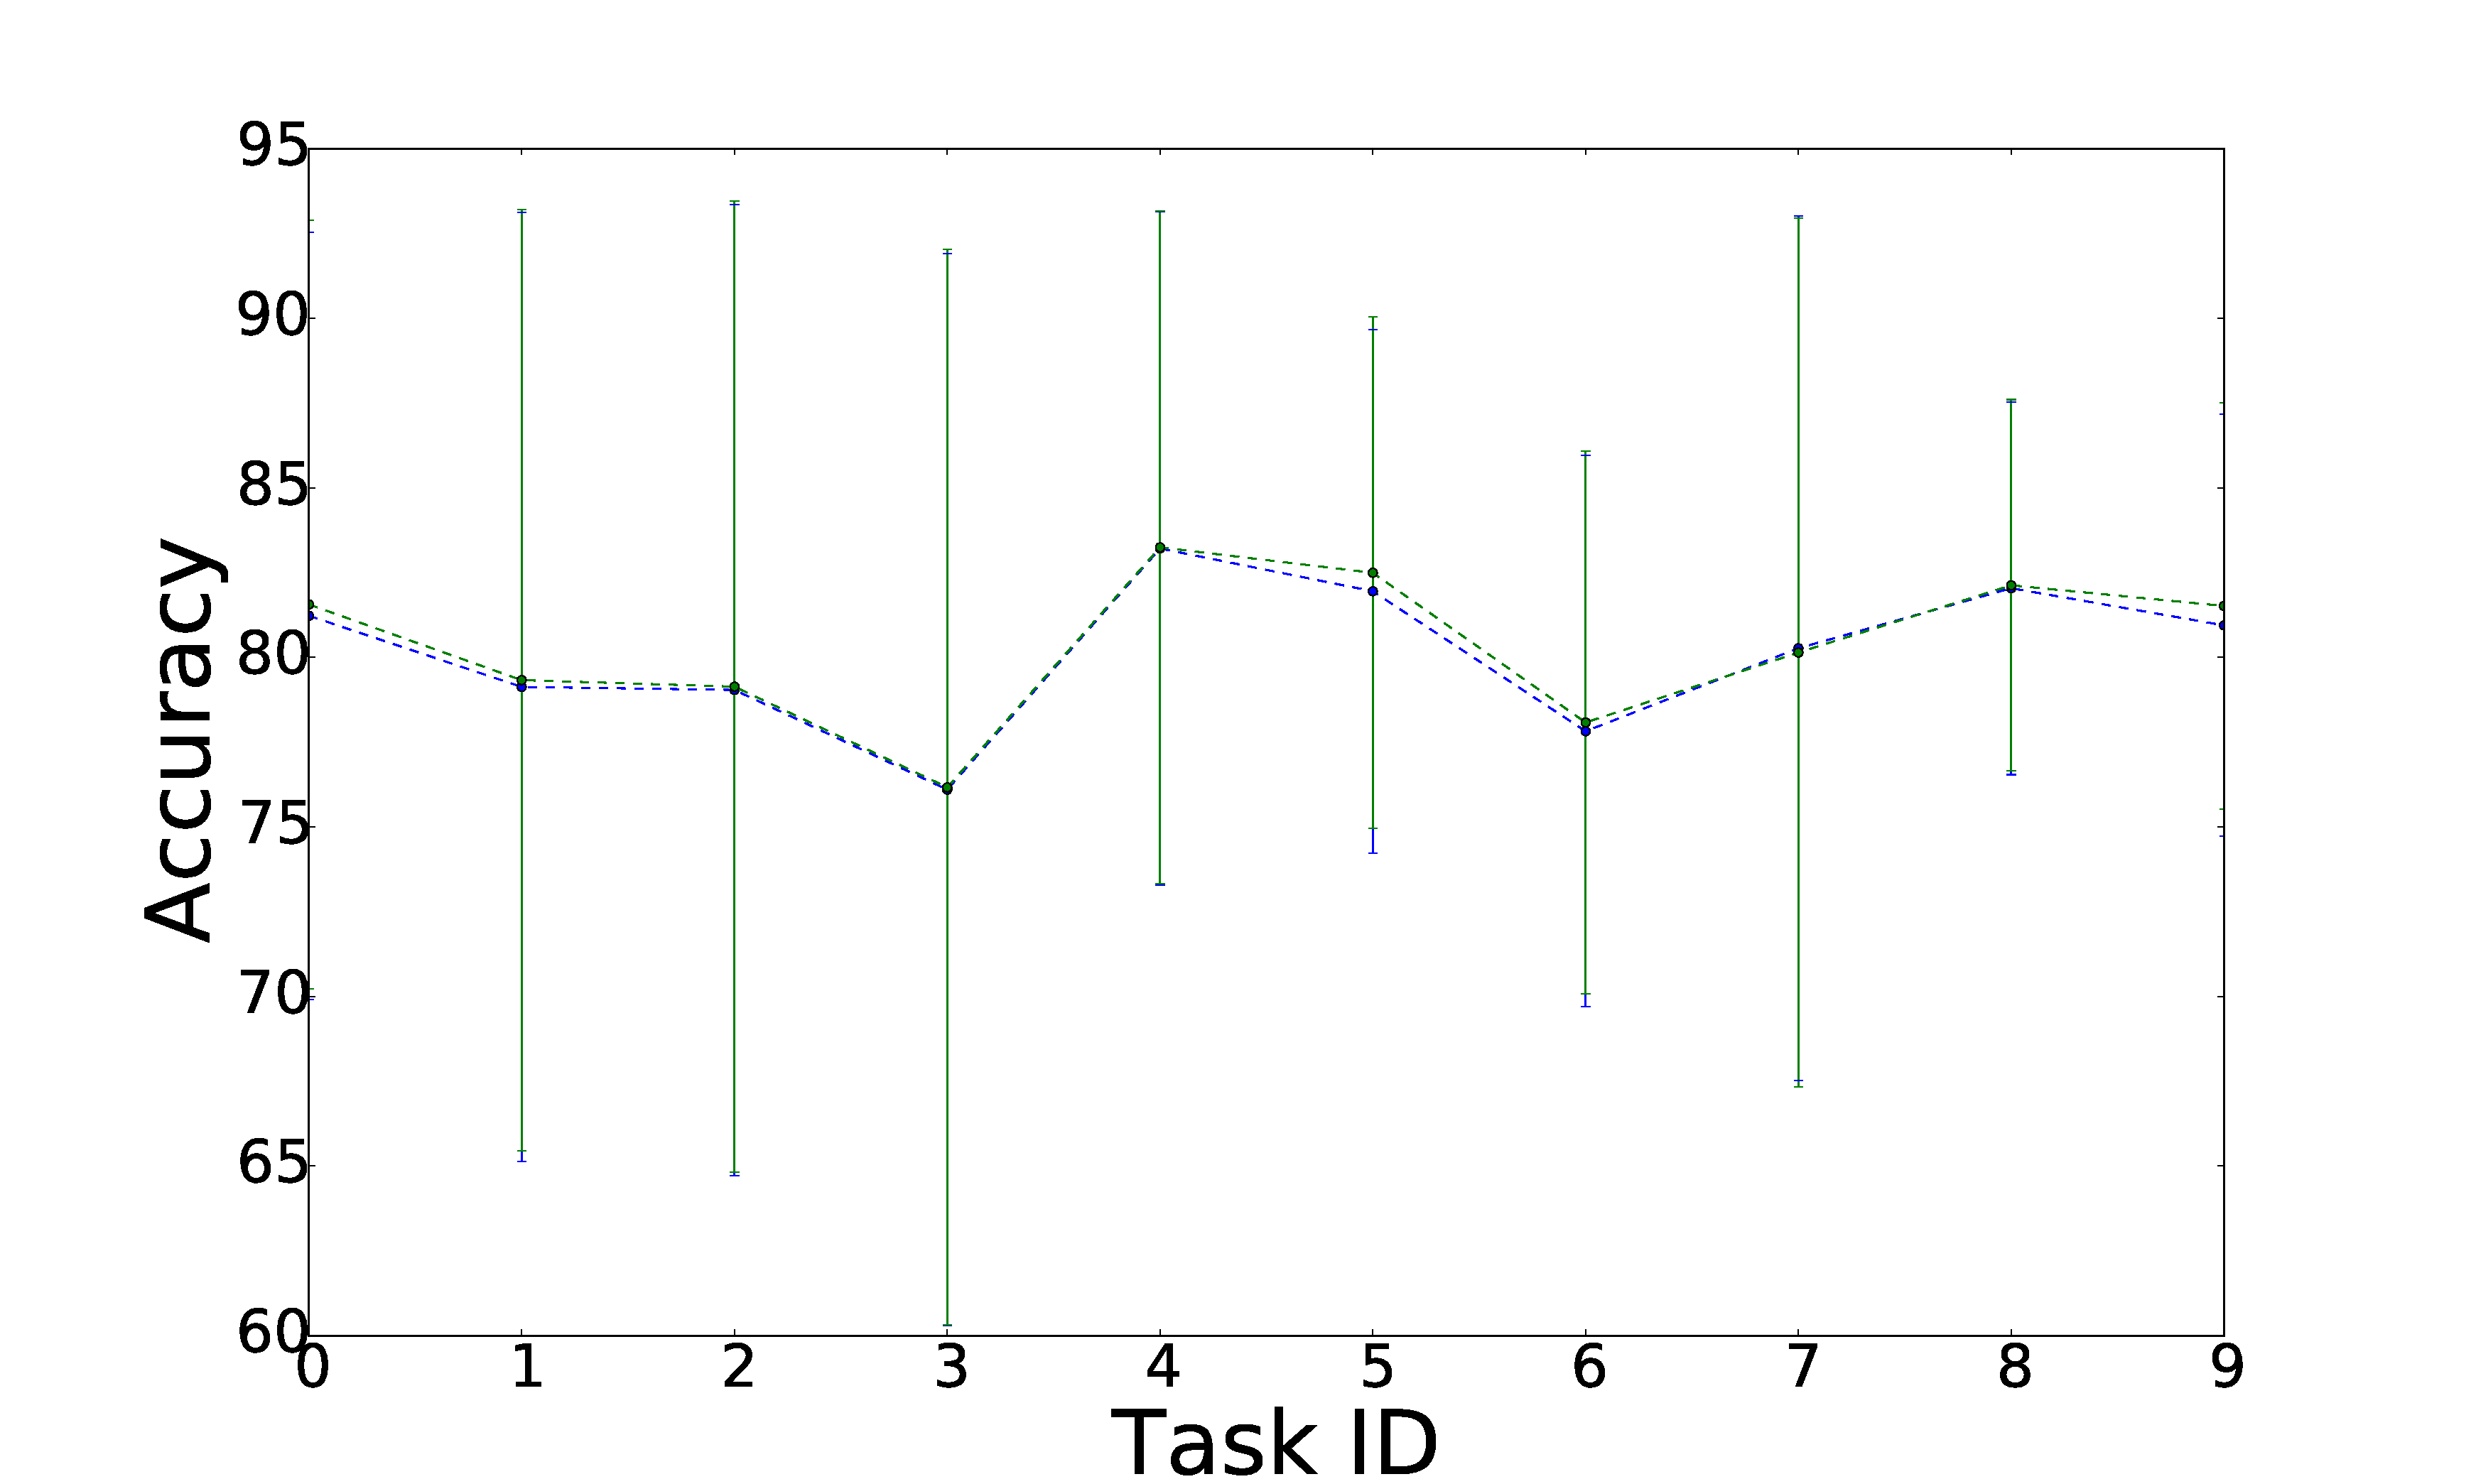
\includegraphics[width=\textwidth]{figures/comp_average_mlp}
        \caption{Neural network}
    \end{subfigure}
    \caption{Comparison with baseline}
    \label{fig:baseline}
\end{figure}


\subsection{Comparison of sparse and dense weight vectors}

In this subsection we test the performance penalty of enforcing sparsity on the annotator weight vectors. We evaluate our assumption that a low number of high-quality annotators can together incur high performance. This turns out to be true, according to our results, shown on \autoref{fig:sparsity}.

\begin{figure}[!htb]
    \centering
    \begin{subfigure}[b]{0.45\textwidth}
        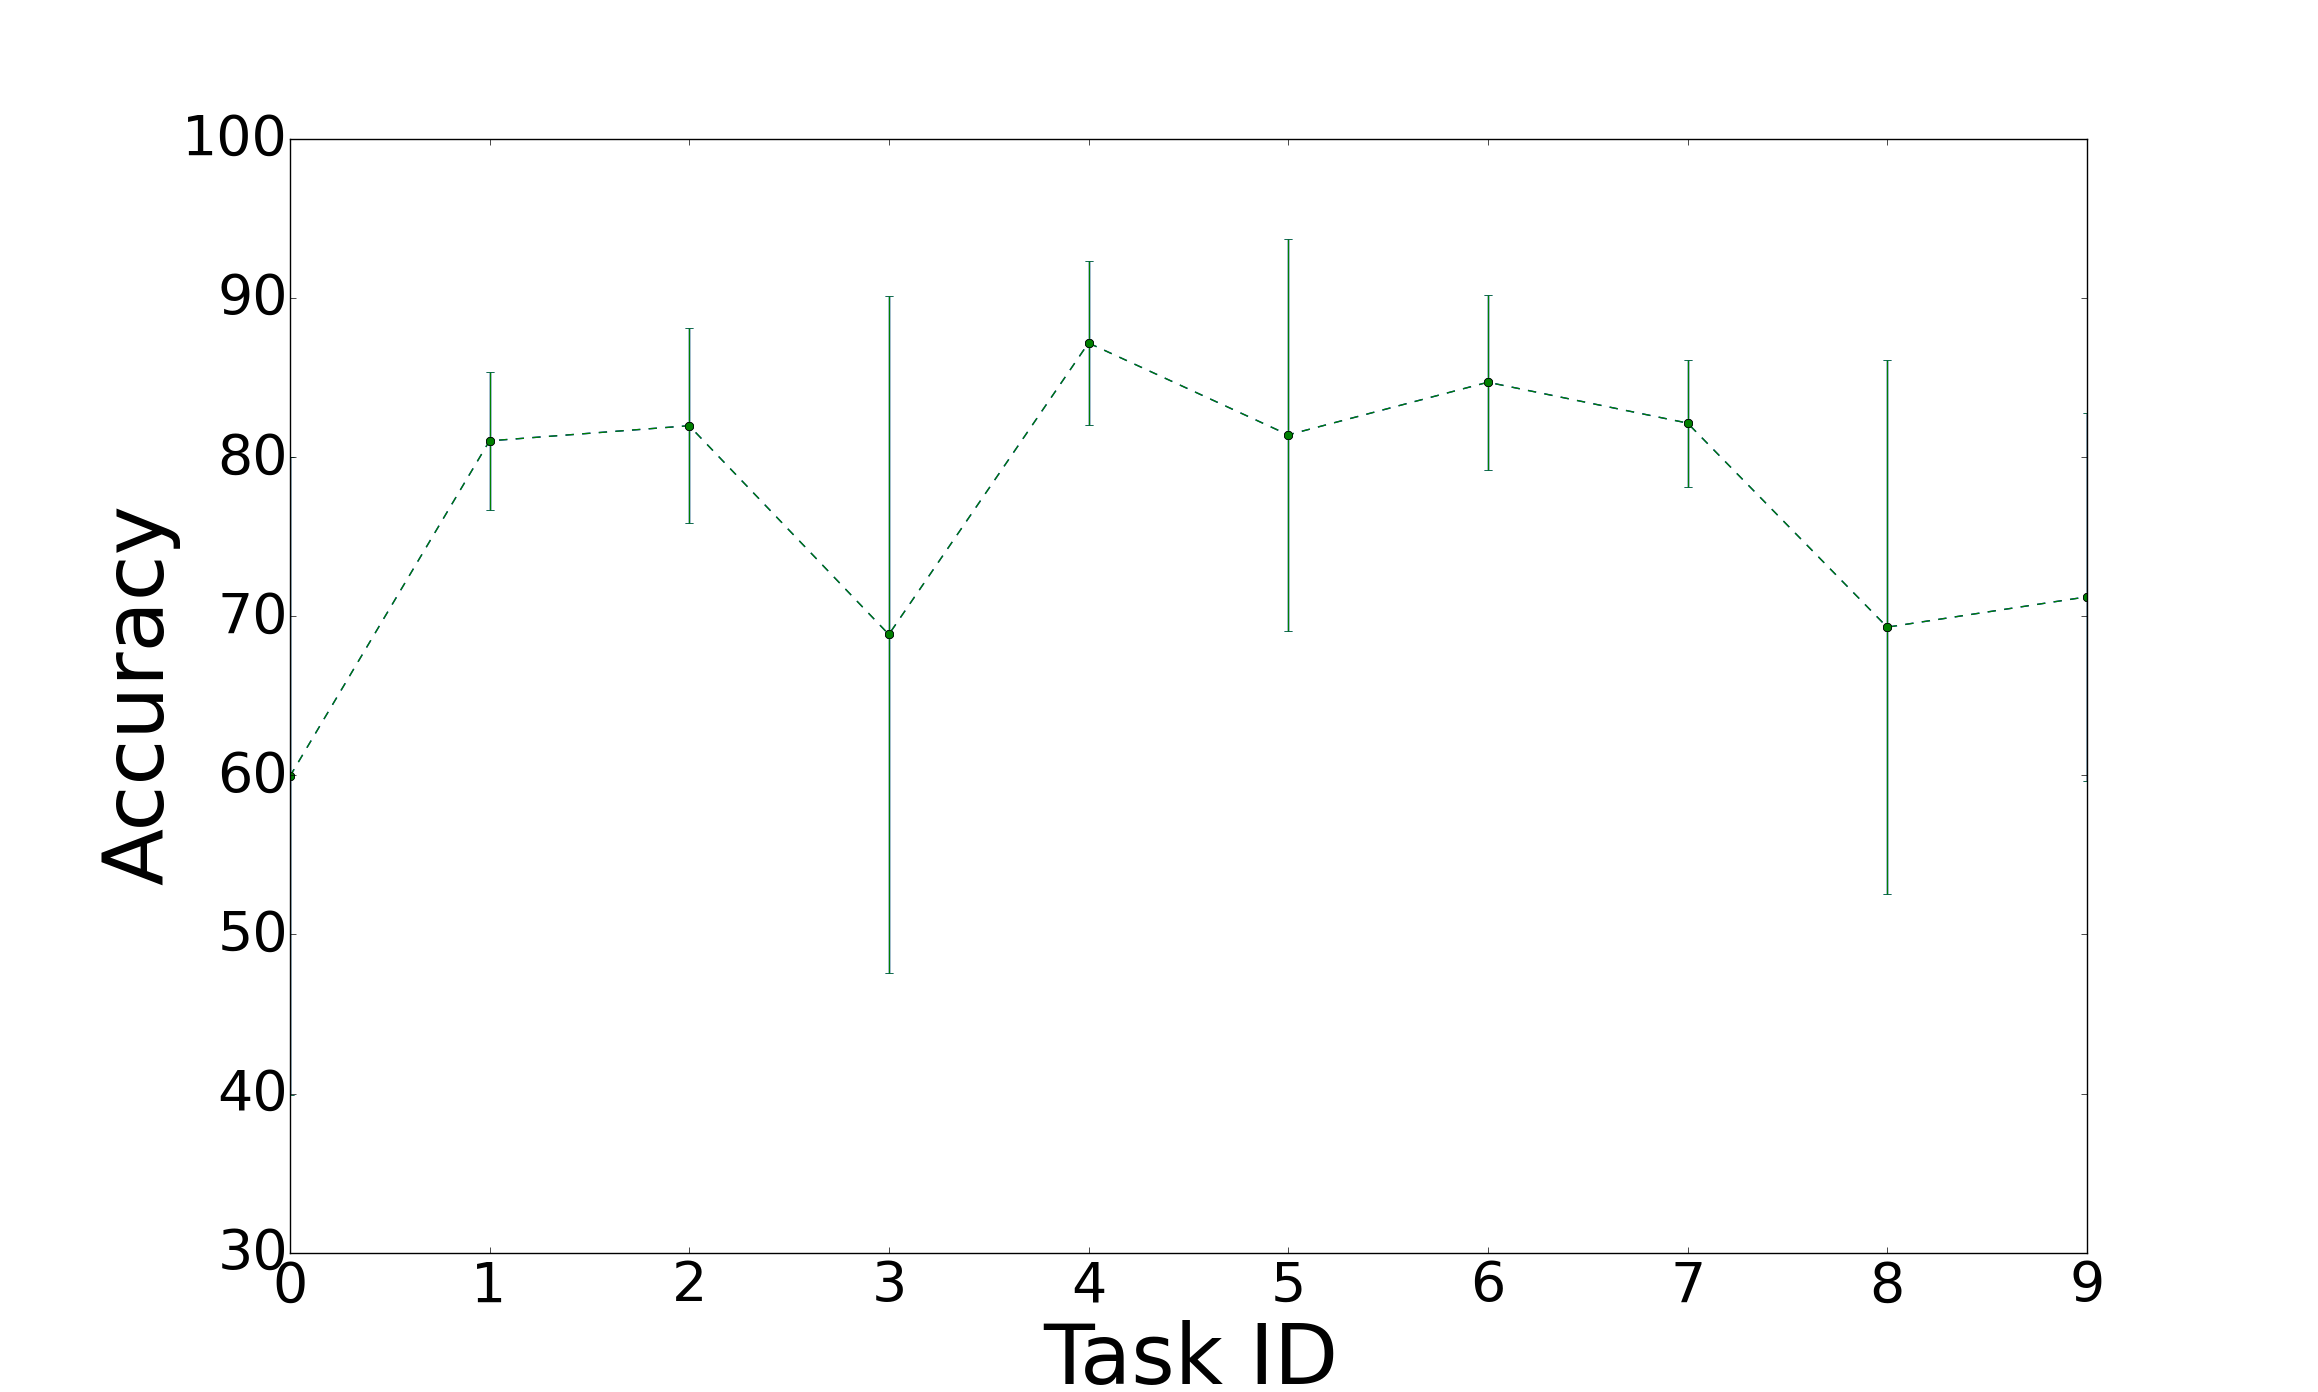
\includegraphics[width=\textwidth]{figures/plot_mlp}
        \caption{Logistic regression}
    \end{subfigure}
    \begin{subfigure}[b]{0.45\textwidth}
        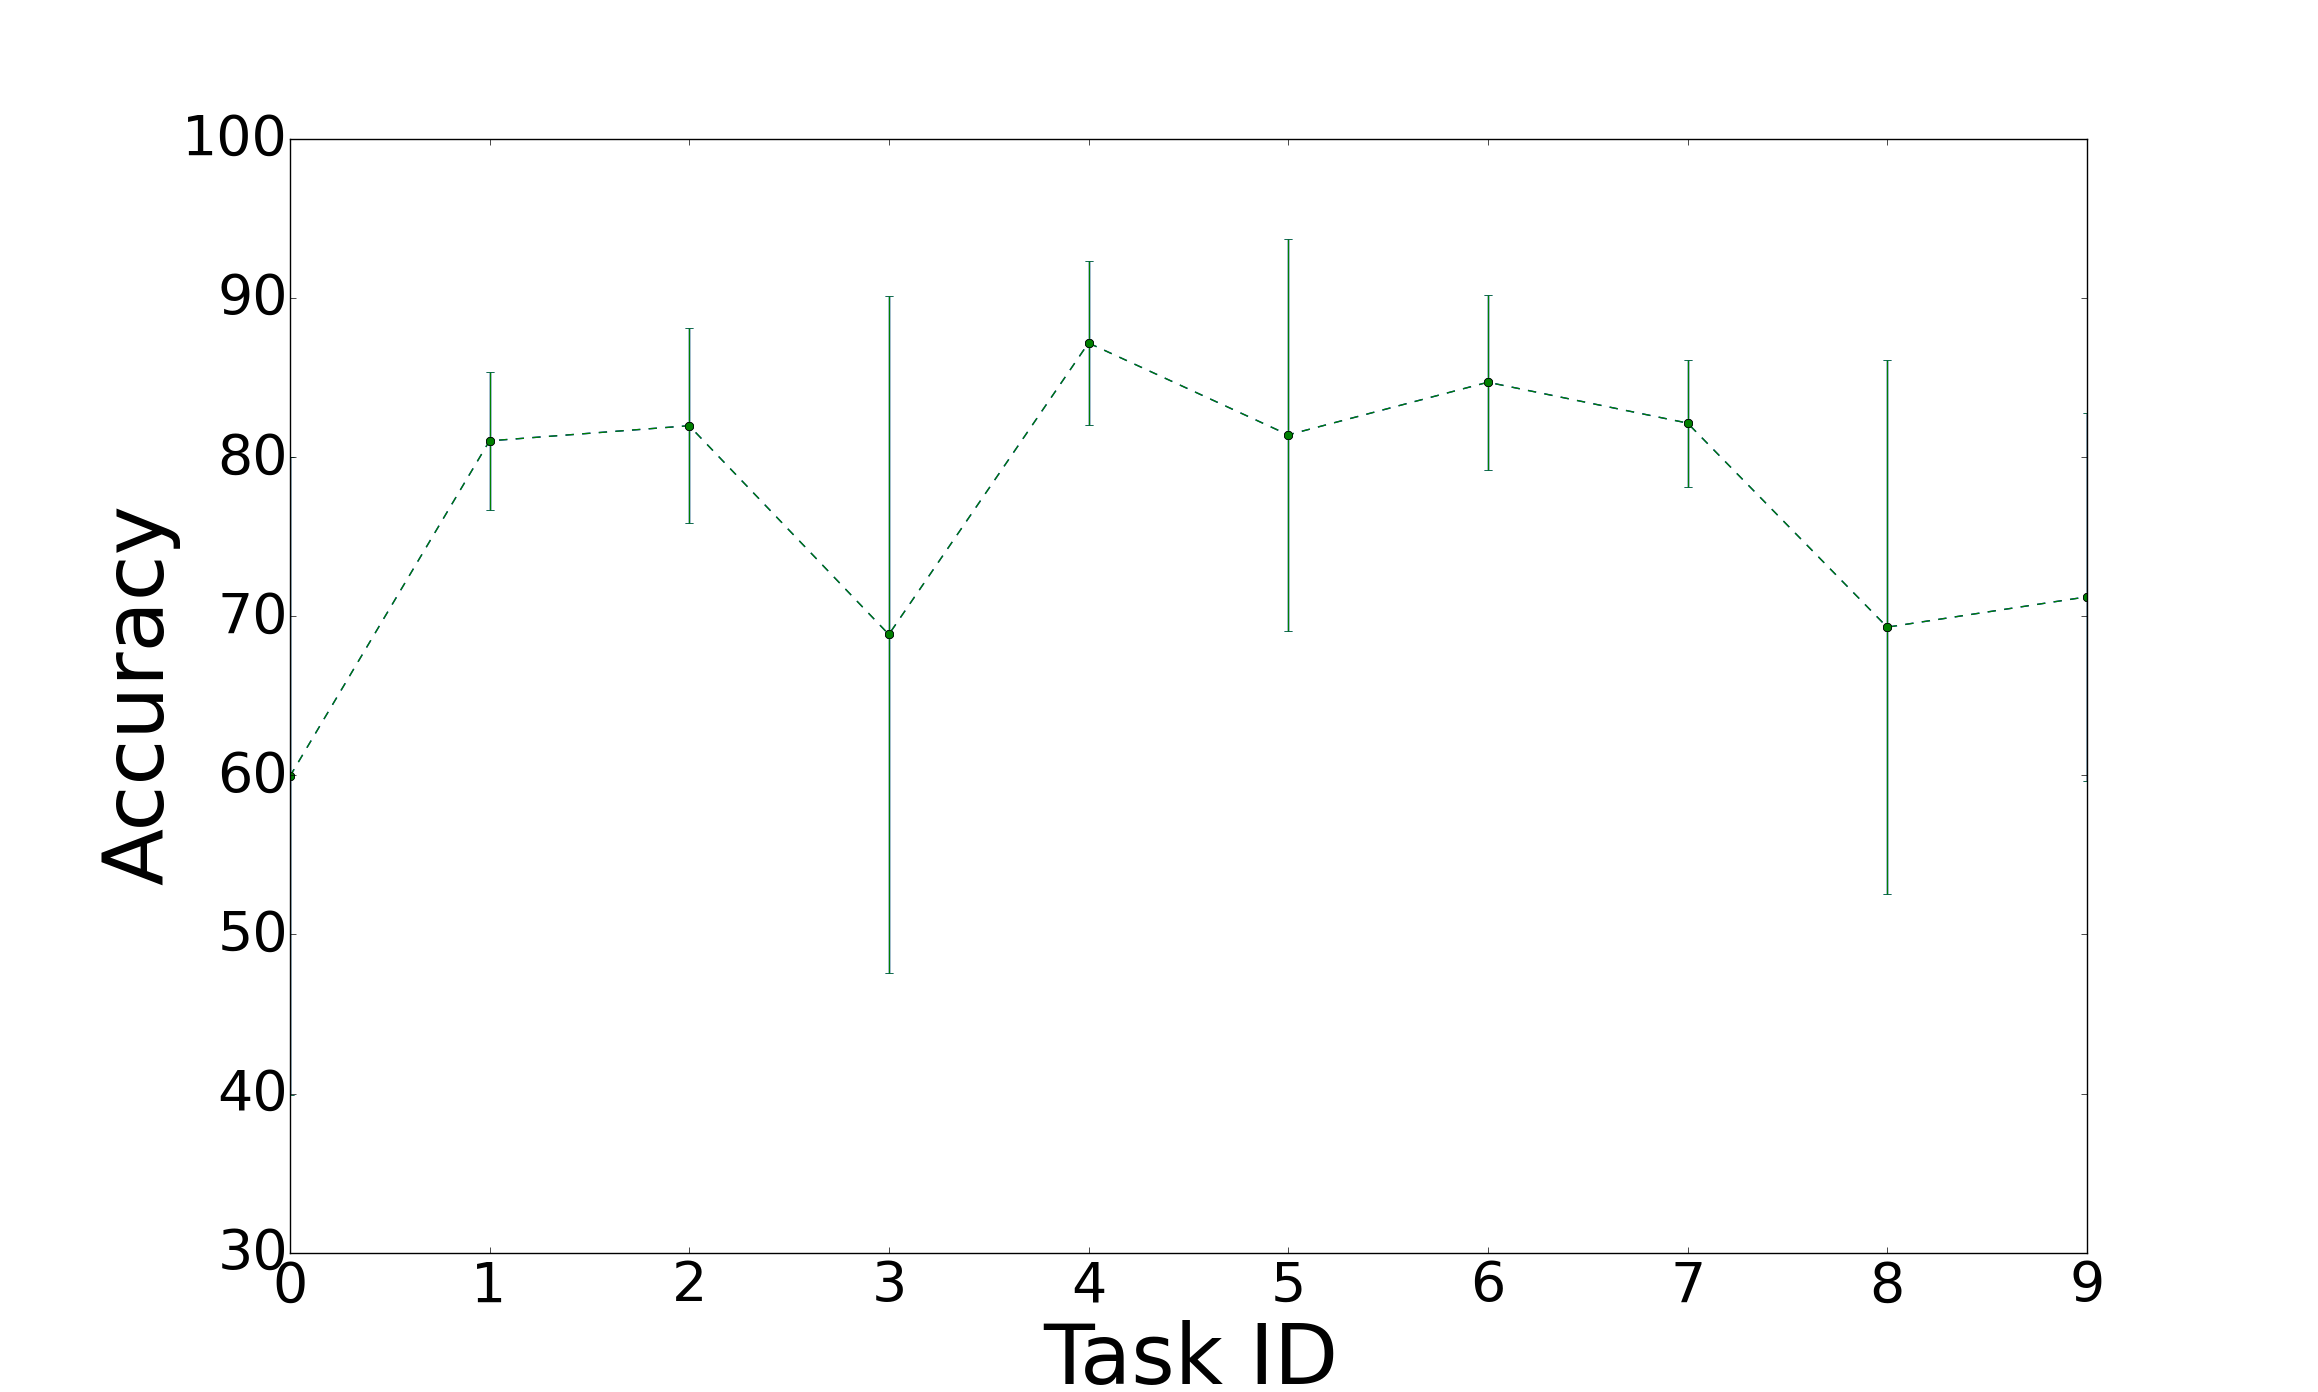
\includegraphics[width=\textwidth]{figures/plot_mlp}
        \caption{Neural network}
    \end{subfigure}
    \caption{Effect of sparsity on model accuracy}
    \label{fig:sparsity}
\end{figure}


\subsection{Sensitivity to the weight of the regularization}

In the beginning, we examine the changes of the loss function when increasing the parameter $\lambda$ from 0 to 1, thereby adding the weight to the sparsity part of the loss function. The results of this test are displayed on \autoref{fig:sensitivity}.

\begin{figure}[!htb]
    \centering
    \begin{subfigure}[b]{0.45\textwidth}
        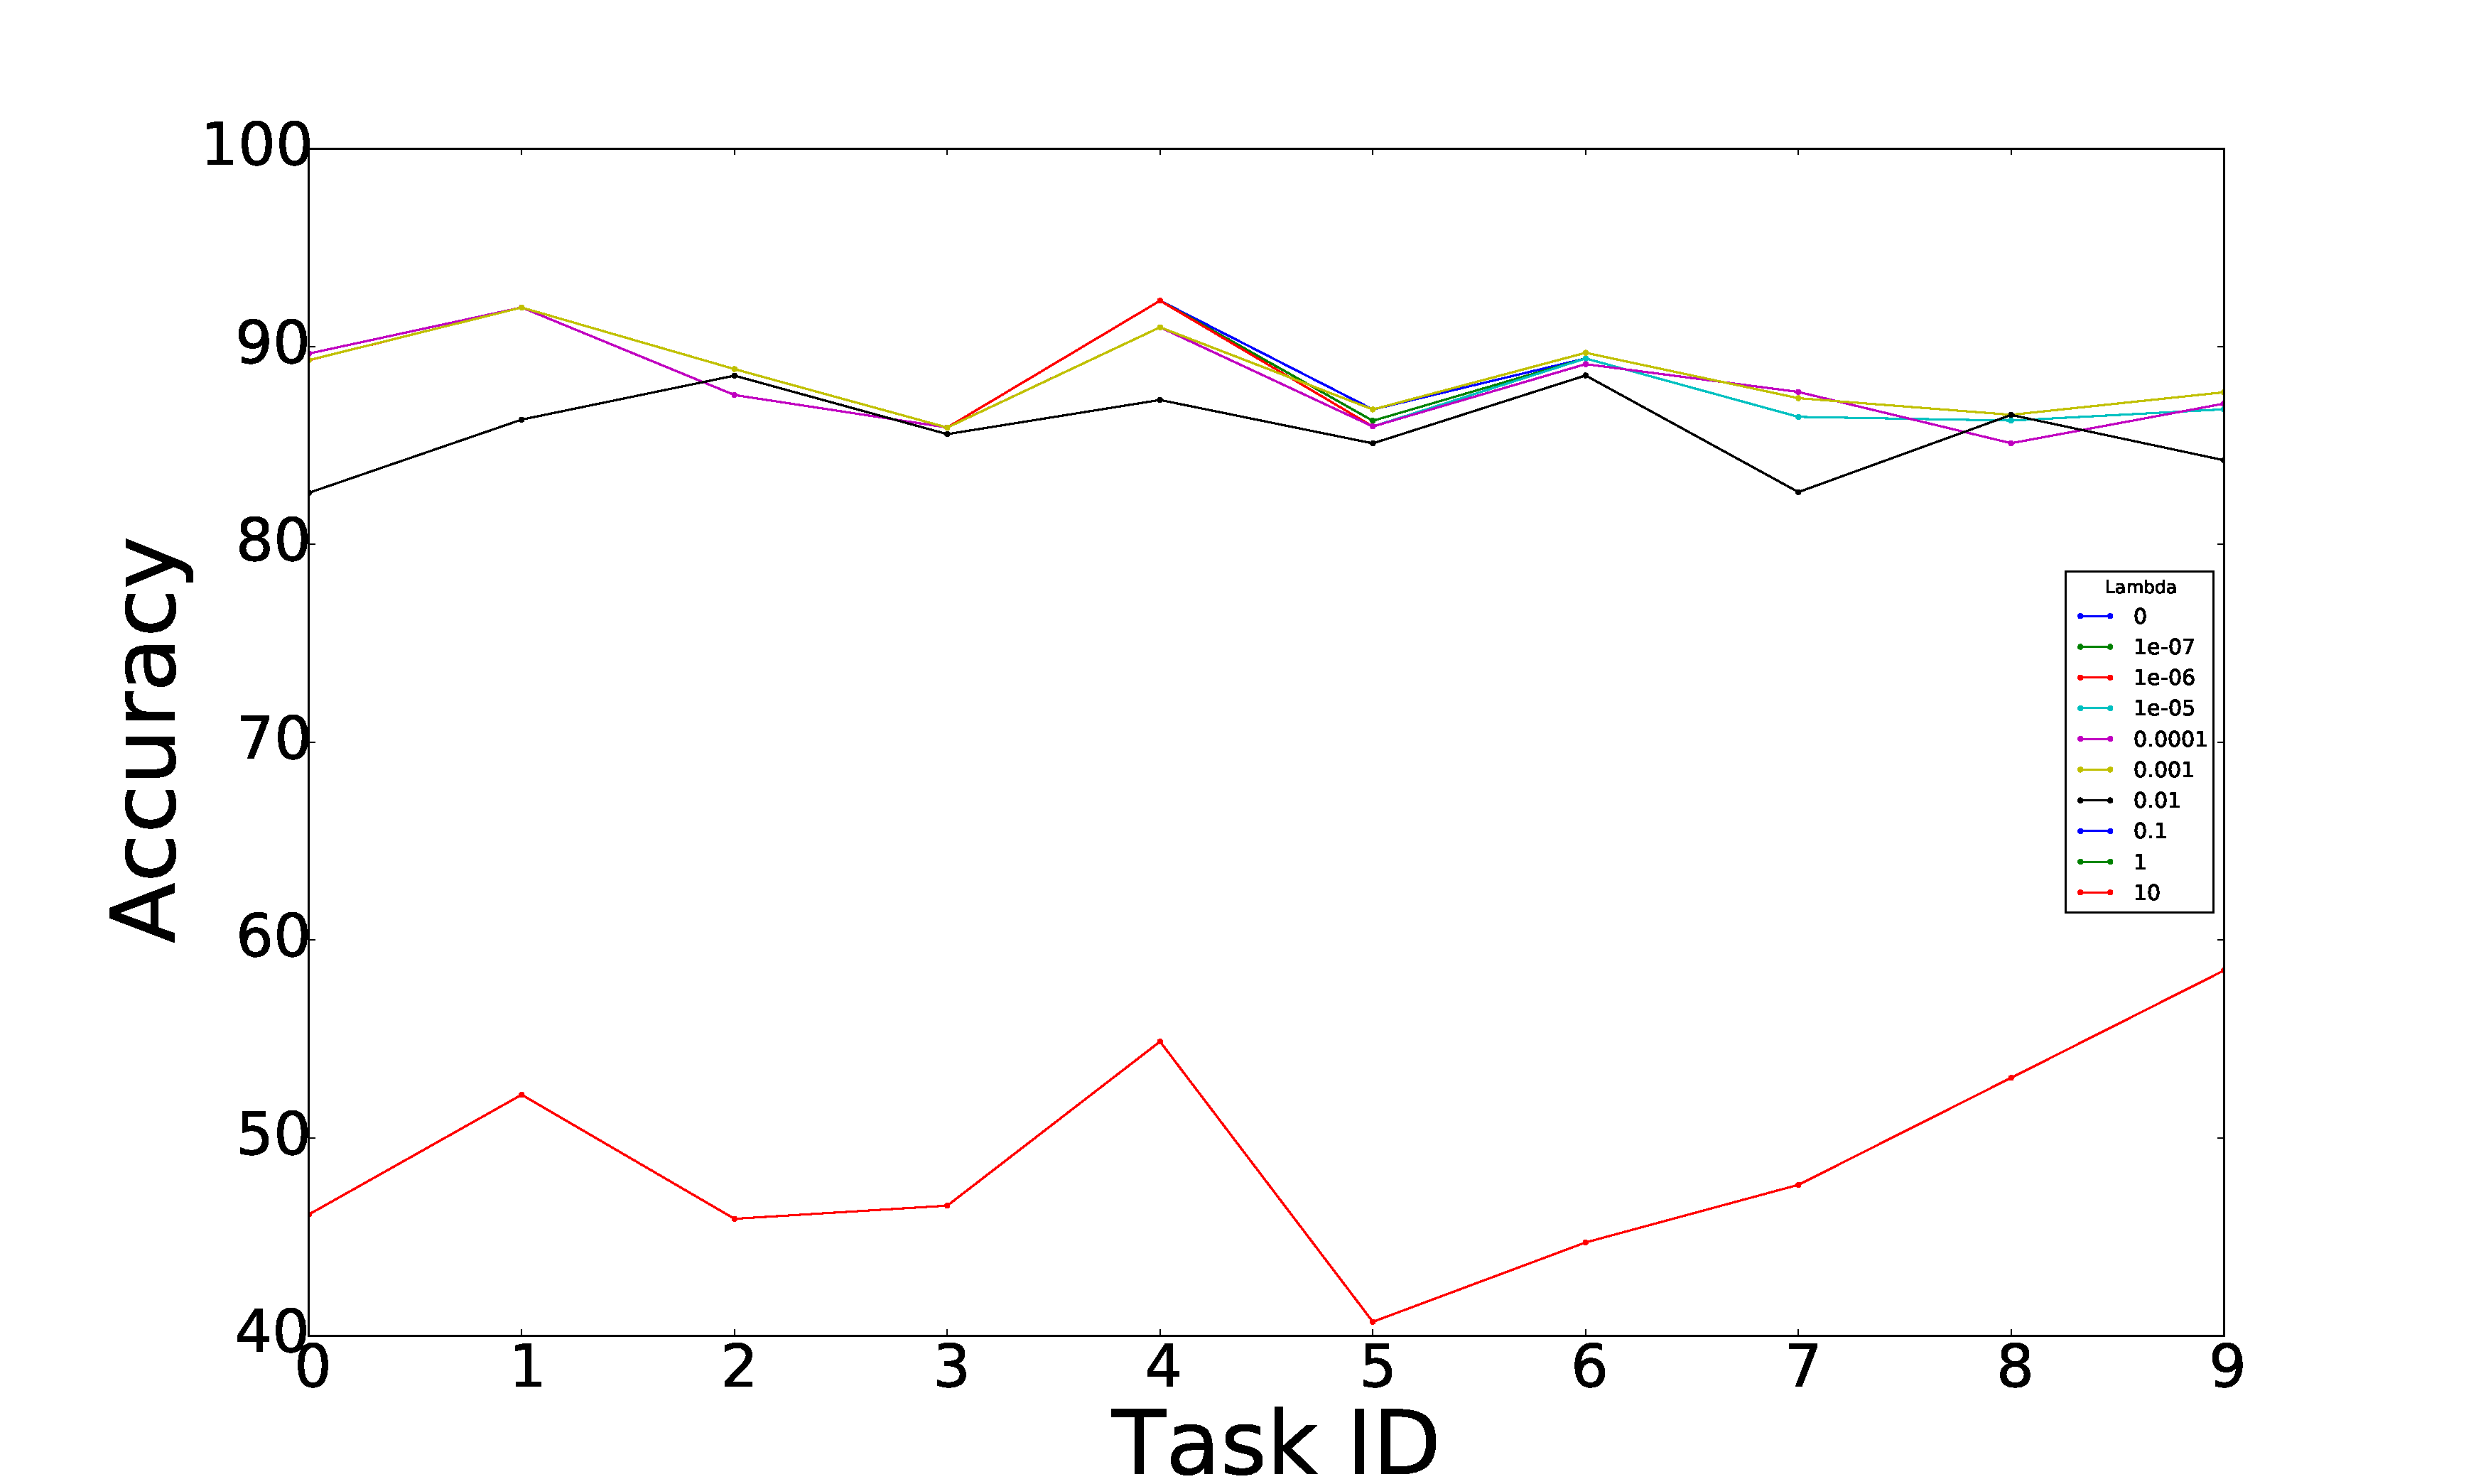
\includegraphics[width=\textwidth]{figures/accuracy_lambda}
        \caption{Logistic regression}
    \end{subfigure}
    \begin{subfigure}[b]{0.45\textwidth}
        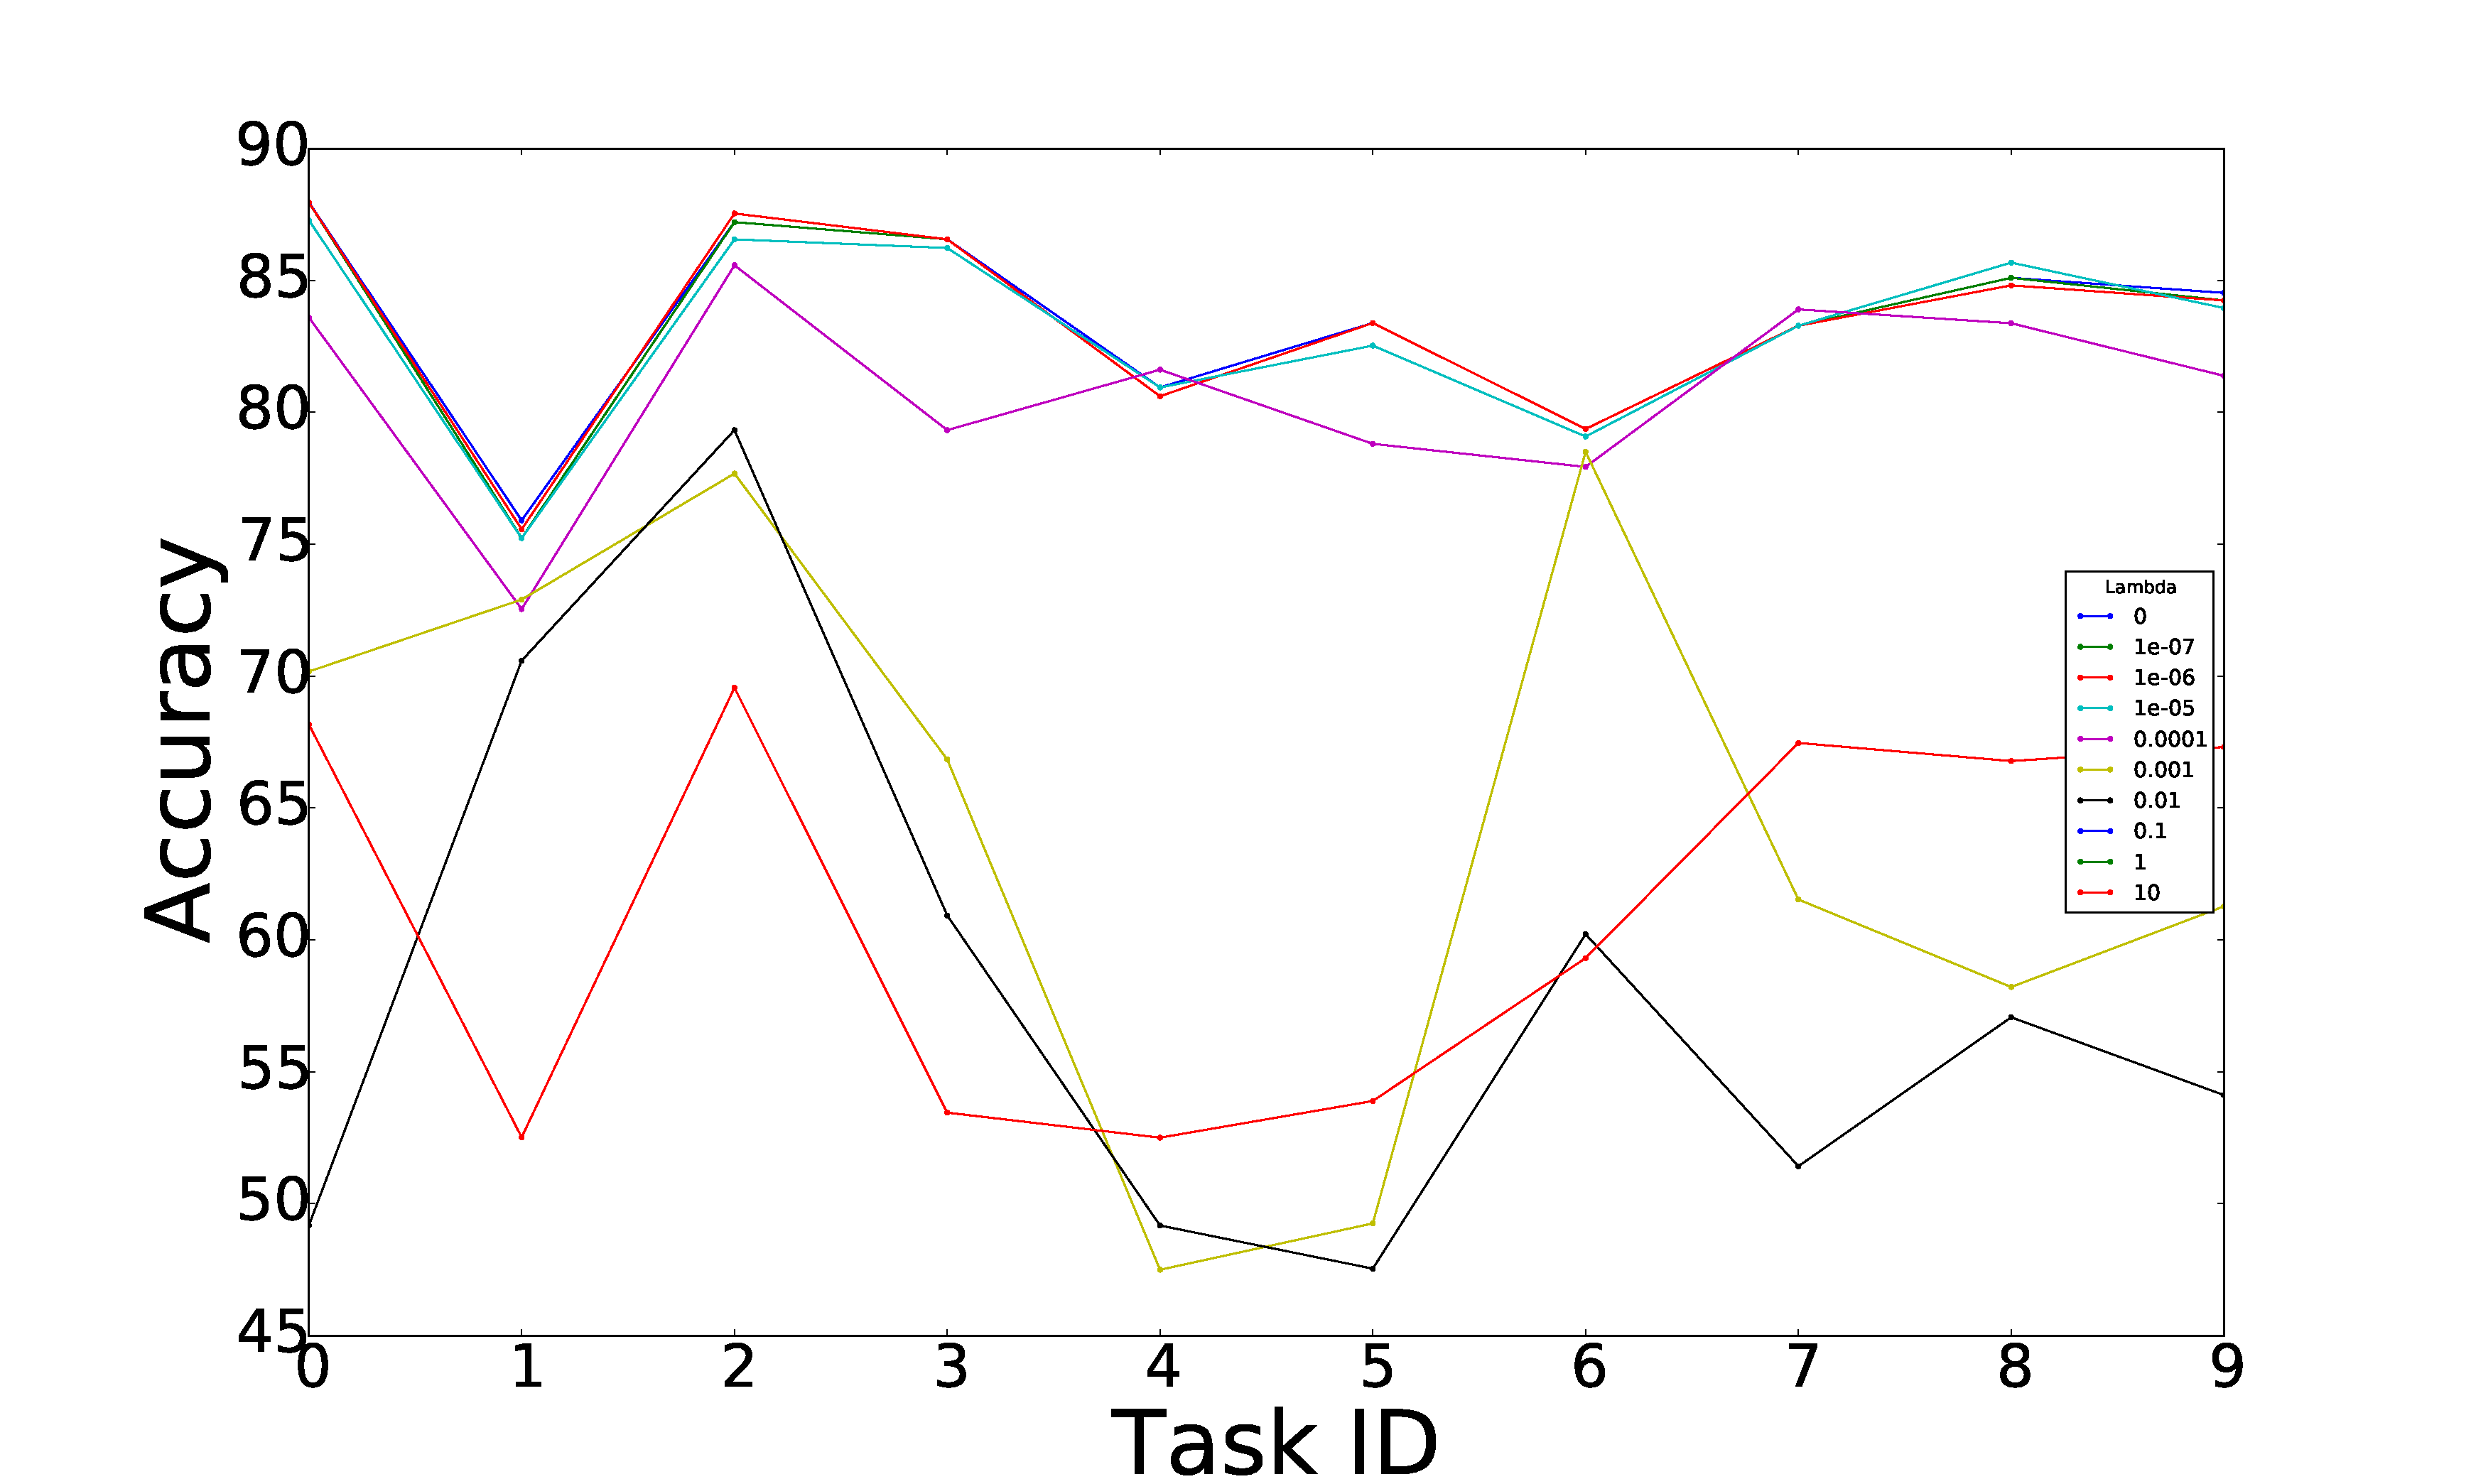
\includegraphics[width=\textwidth]{figures/accuracy_lambda_mlp}
        \caption{Neural network}
    \end{subfigure} 
  \caption{Sensitivity to the hyperparameter}
  \label{fig:sensitivity}
\end{figure}




\subsection{Accuracy on synthetic data}

In this subsection we show the classification performance on our synthetically generated data. We show on \autoref{fig:synthetic}.that a small number of efficient labeling experts can give a much higher performance than individual labelers. 

\begin{figure}[!htb]
    \centering
    \begin{subfigure}[b]{0.45\textwidth}
        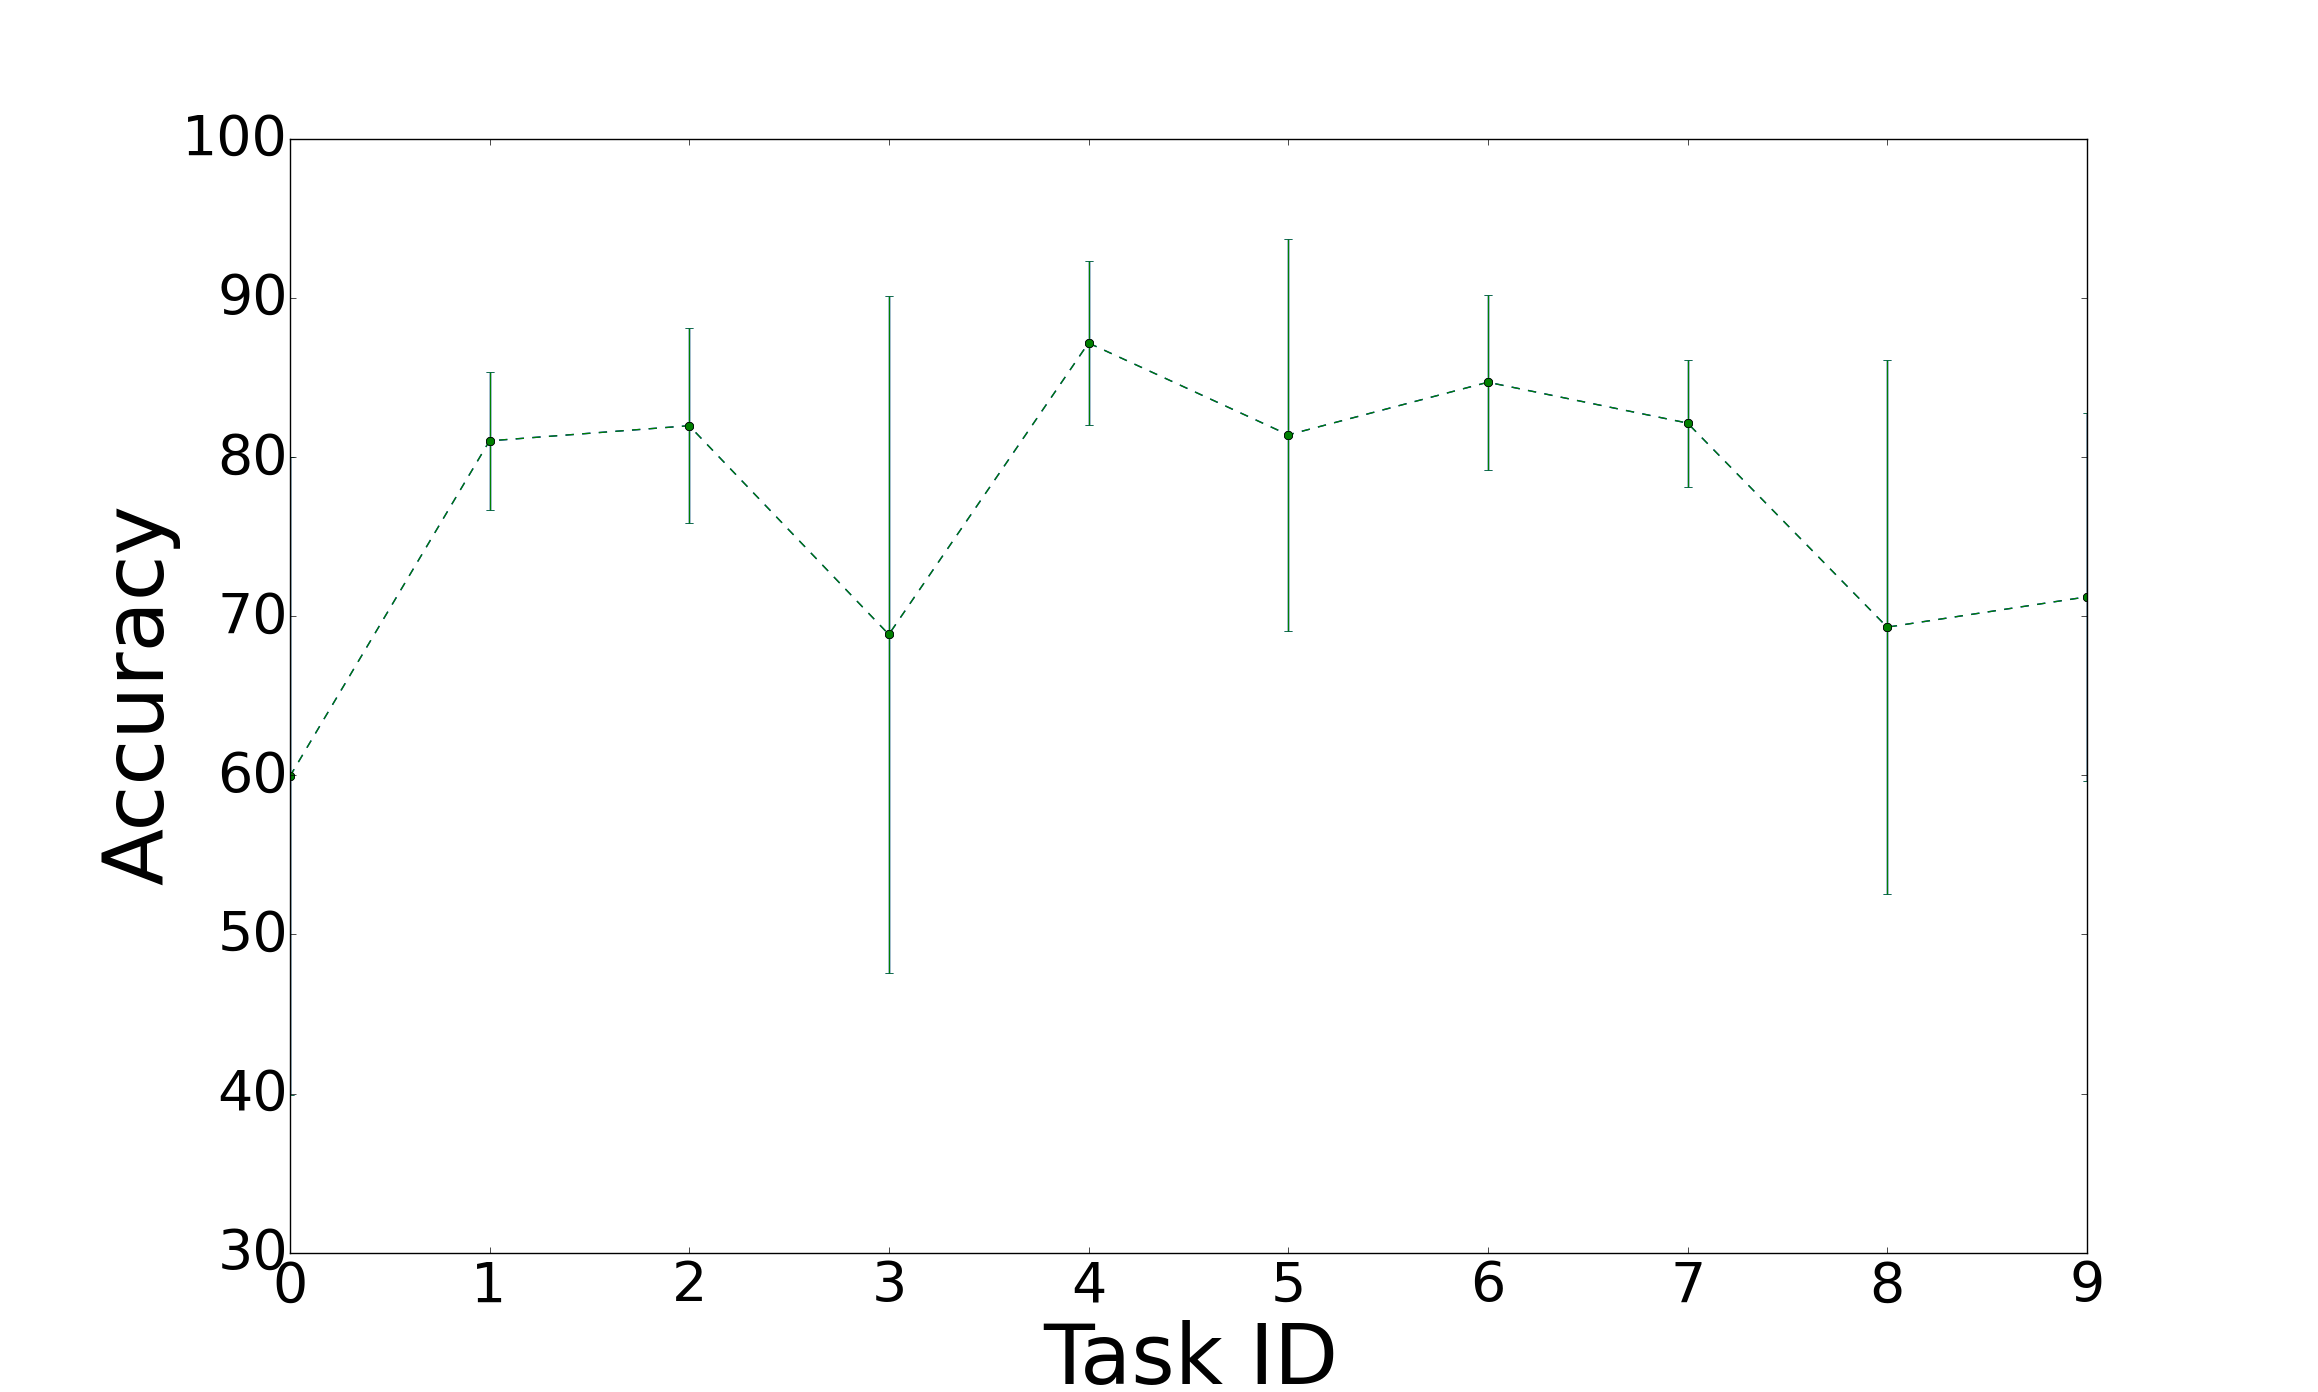
\includegraphics[width=\textwidth]{figures/plot_mlp}
        \caption{Loss minimization}
    \end{subfigure}
    \begin{subfigure}[b]{0.45\textwidth}
        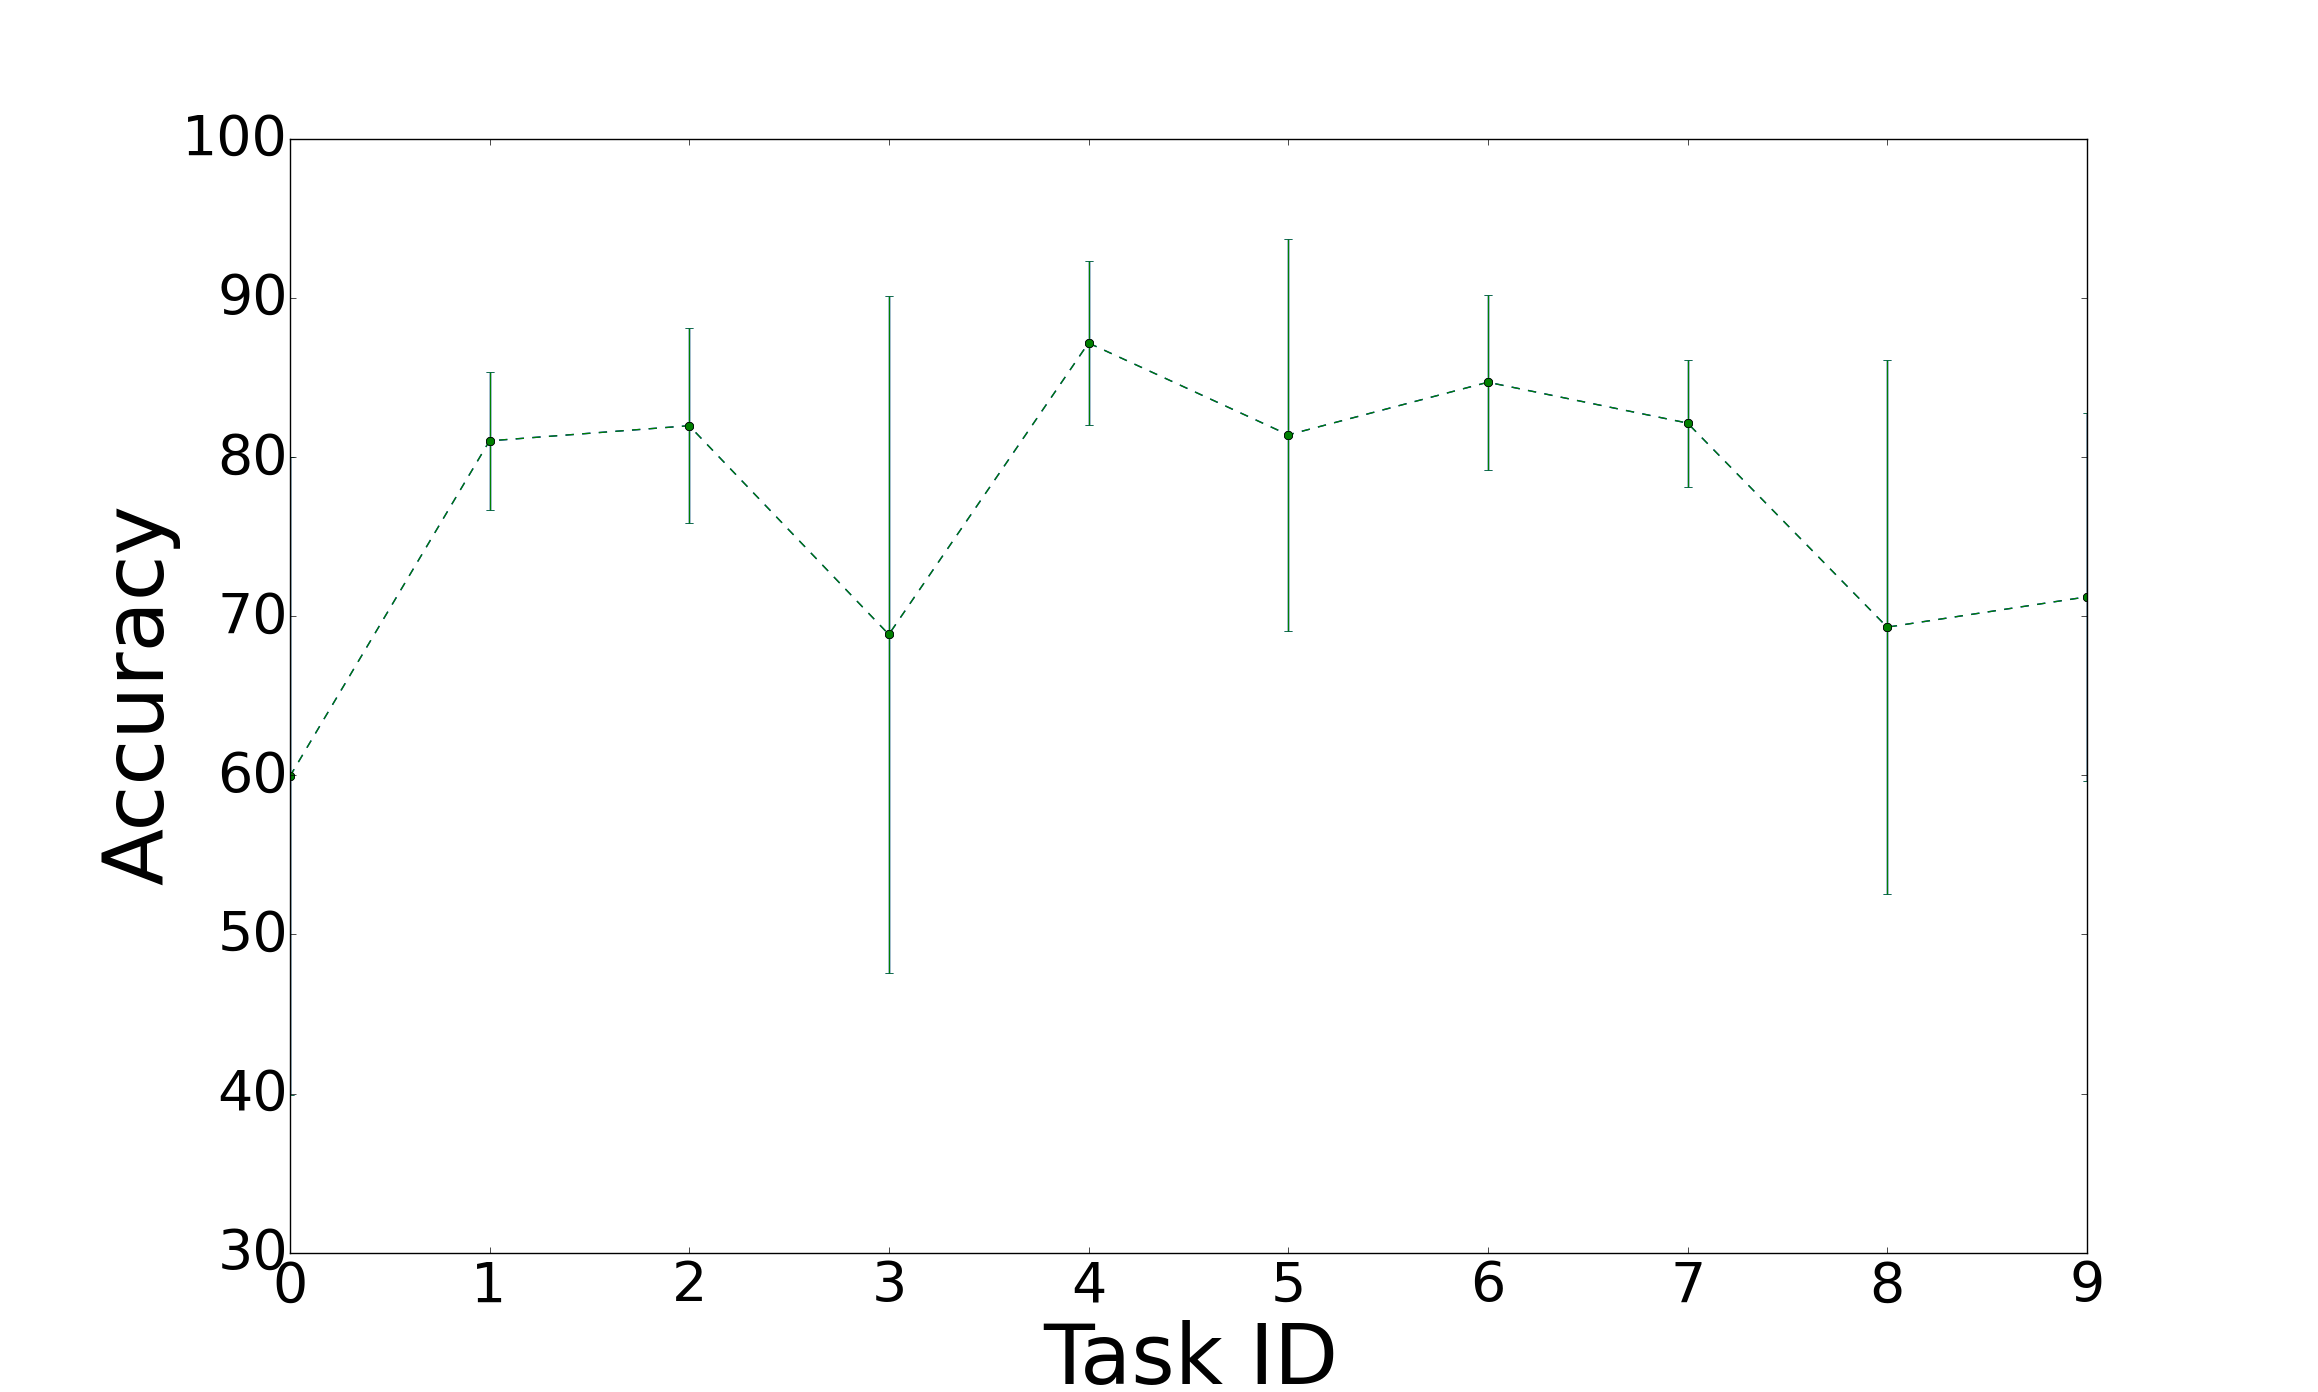
\includegraphics[width=\textwidth]{figures/plot_mlp}
        \caption{Neural Network}
    \end{subfigure}
  \caption{Reduction of annotator subset}
  \label{fig:synthetic}
\end{figure}


\subsection{Comparison of sparse and dense vectors}

In the next figures we show the breakdown of performance for sparse selection w.r.t the selection with no sparsity enforcement. On \autoref{fig:sparsity_mnist} it is noticeable that the error rate is uniform.

\begin{figure}[!htb]
    \centering
    \begin{subfigure}[b]{0.45\textwidth}
        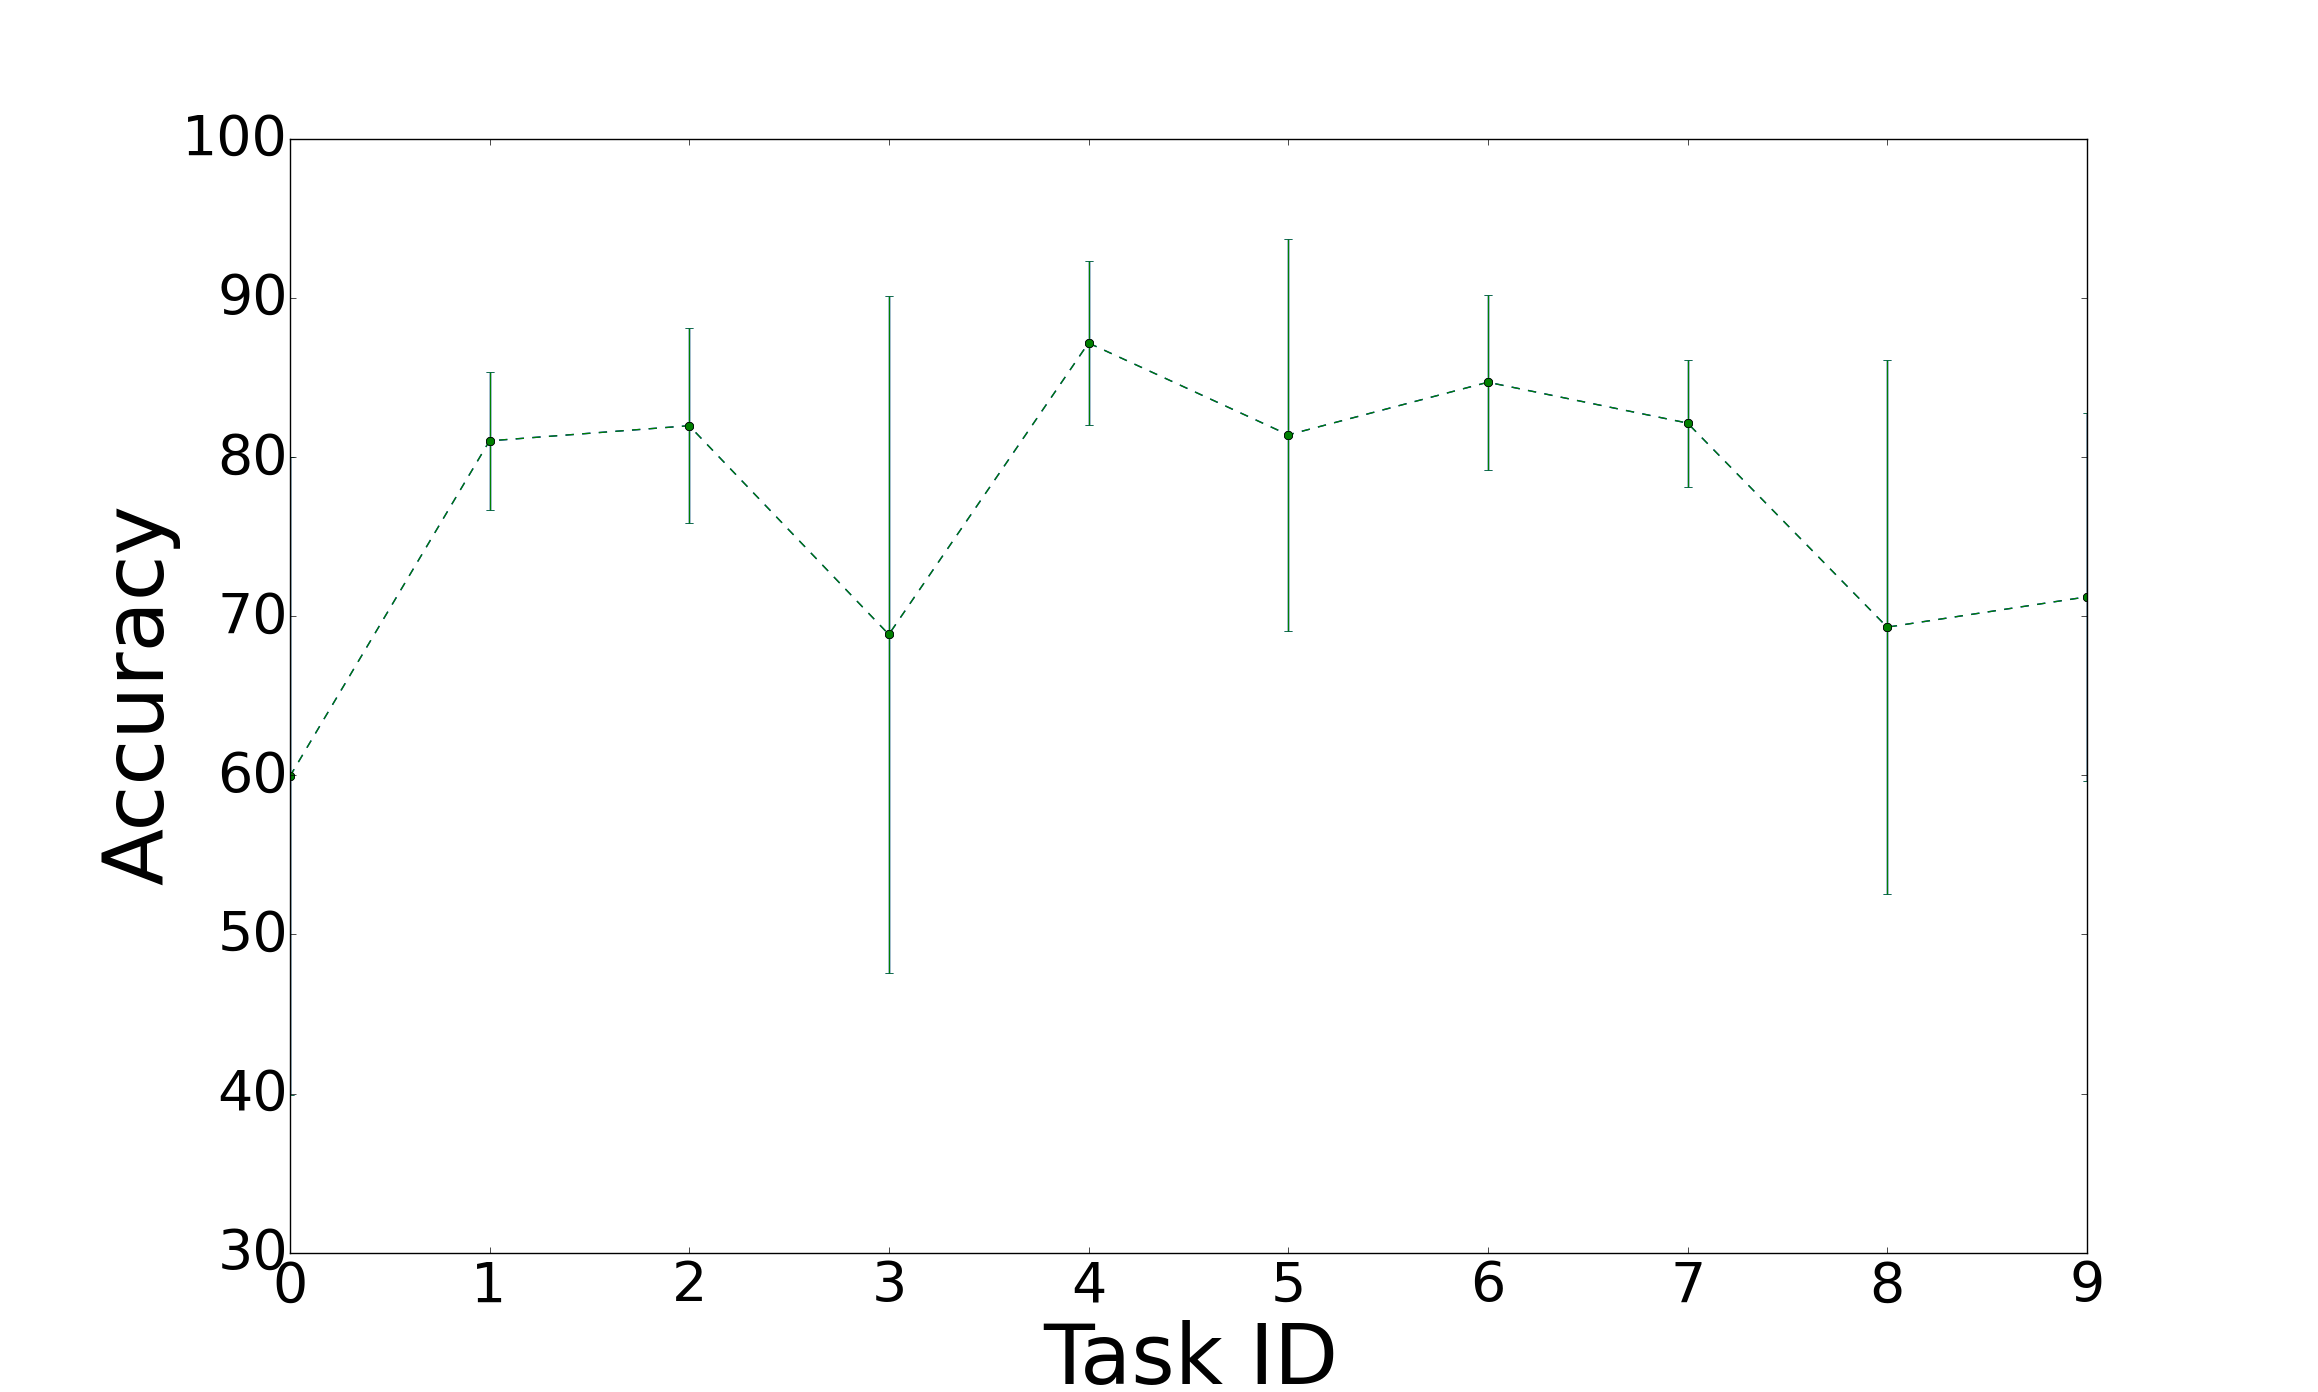
\includegraphics[width=\textwidth]{figures/plot_mlp}
        \caption{Logistic Regression}
    \end{subfigure}
    \begin{subfigure}[b]{0.45\textwidth}
        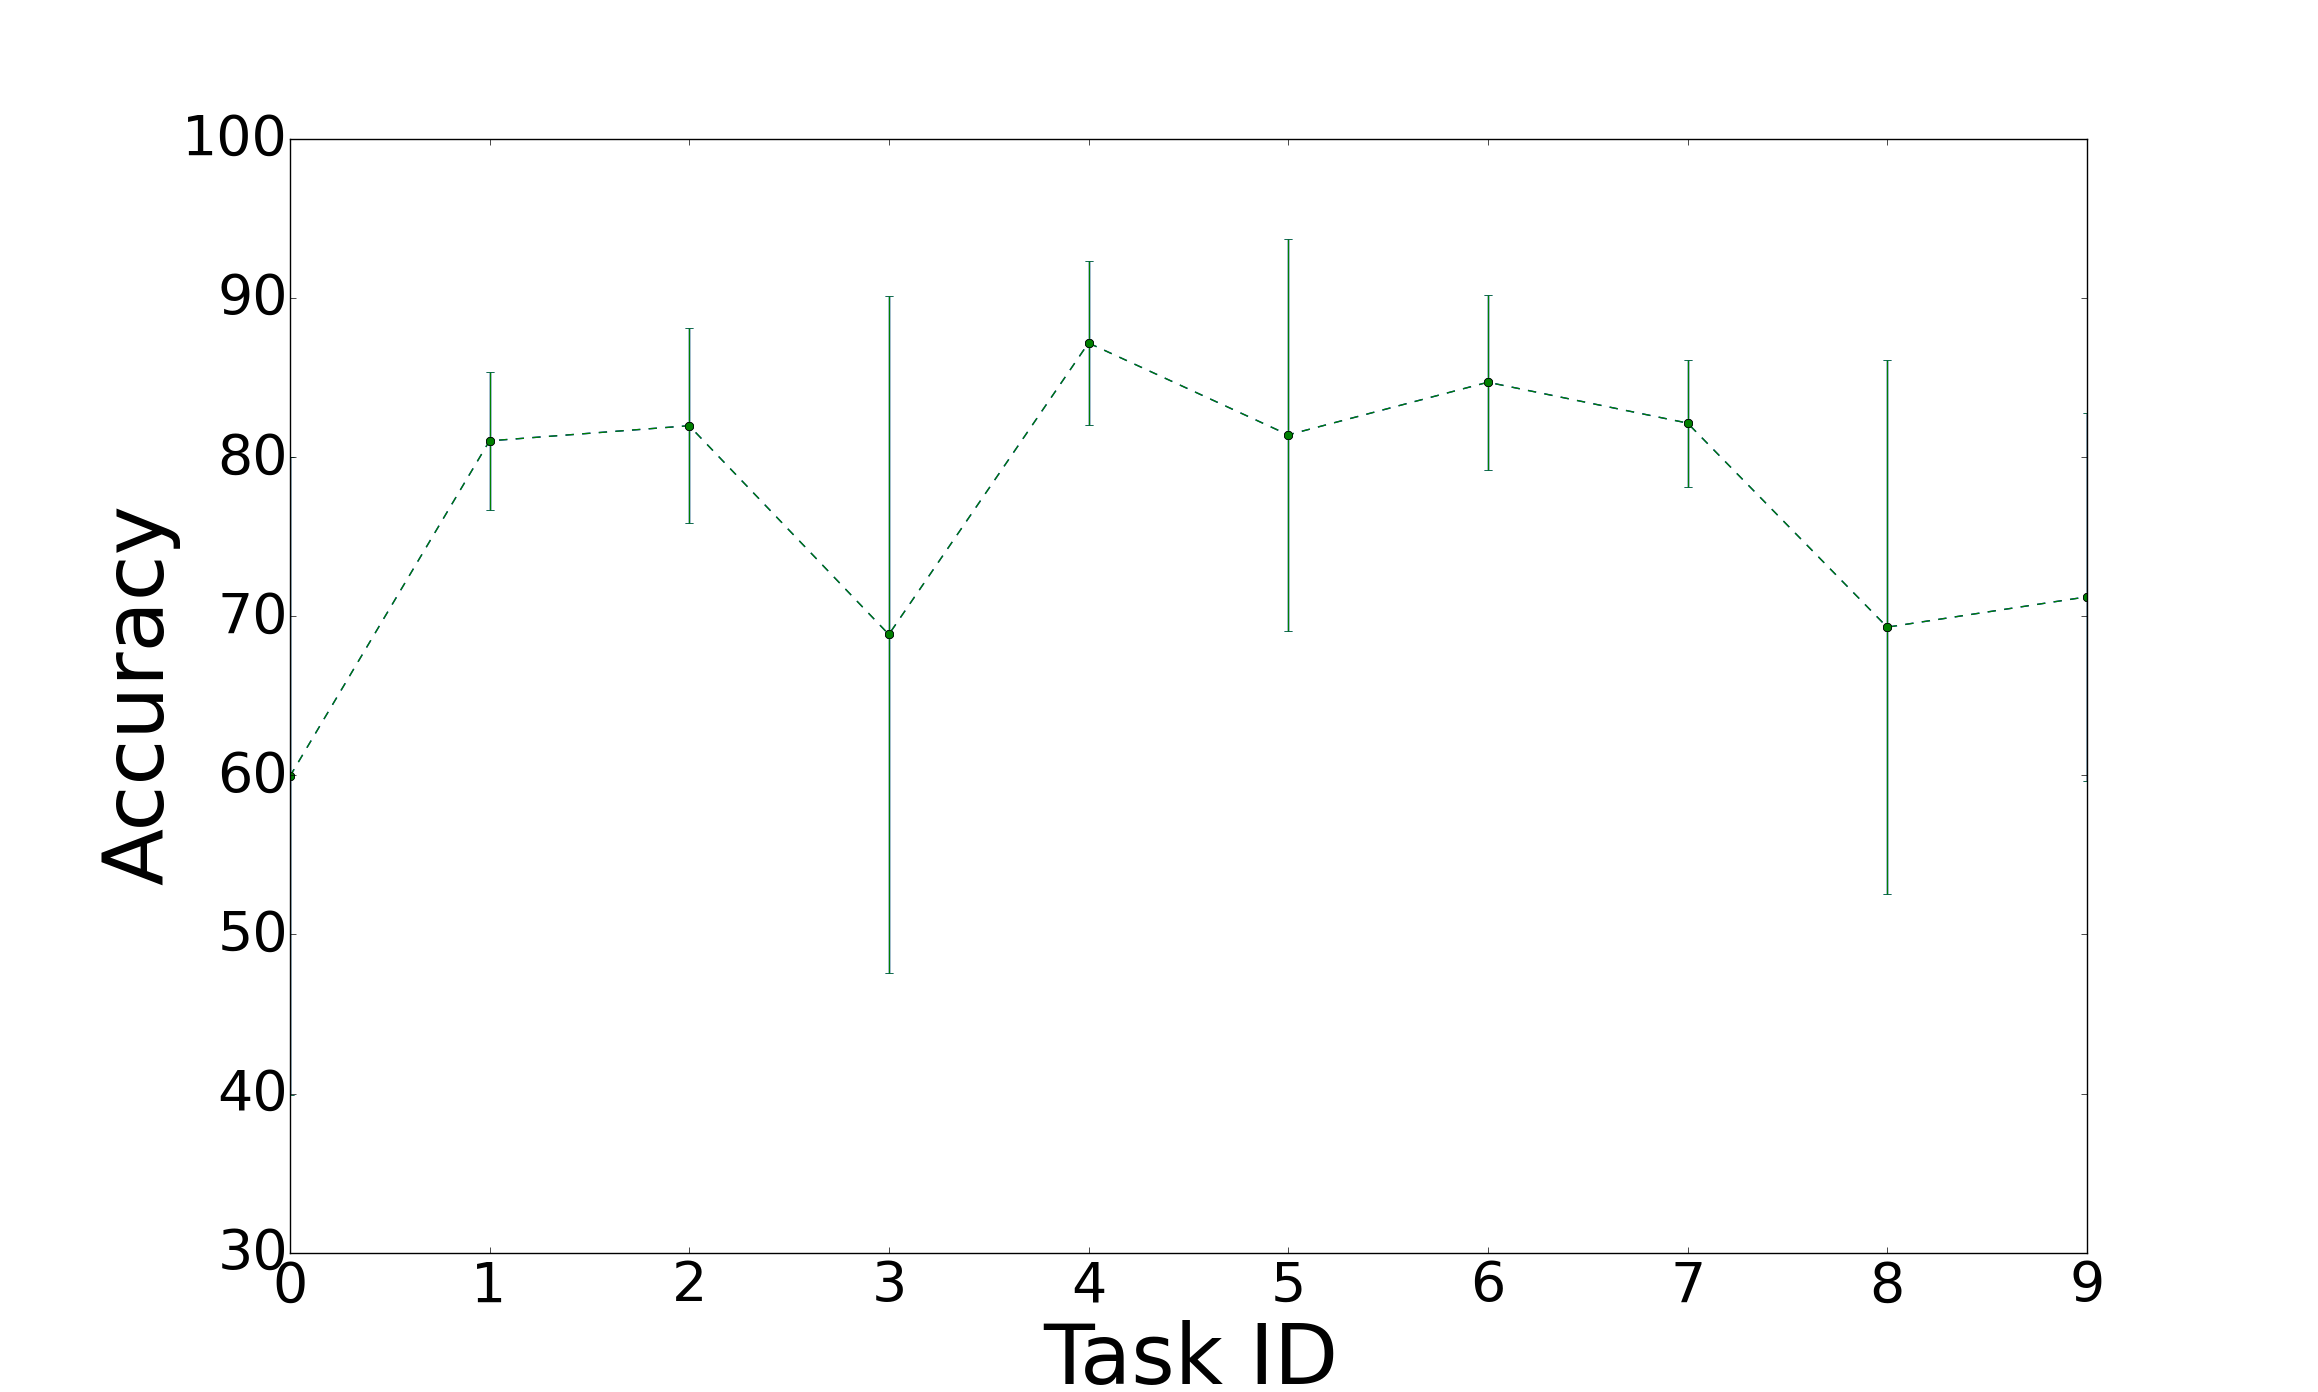
\includegraphics[width=\textwidth]{figures/plot_mlp}
        \caption{Neural Network}
    \end{subfigure}
  \caption{Performance per digit}
  \label{fig:sparsity_mnist}
\end{figure}



\subsection{Size of the annotator set}

In the next group of plots we show how the size of the annotator subset grows with the initial number of annotators. This is shown on  \autoref{fig:subset}

\begin{figure}[!htb]
    \centering
    \begin{subfigure}[b]{0.45\textwidth}
        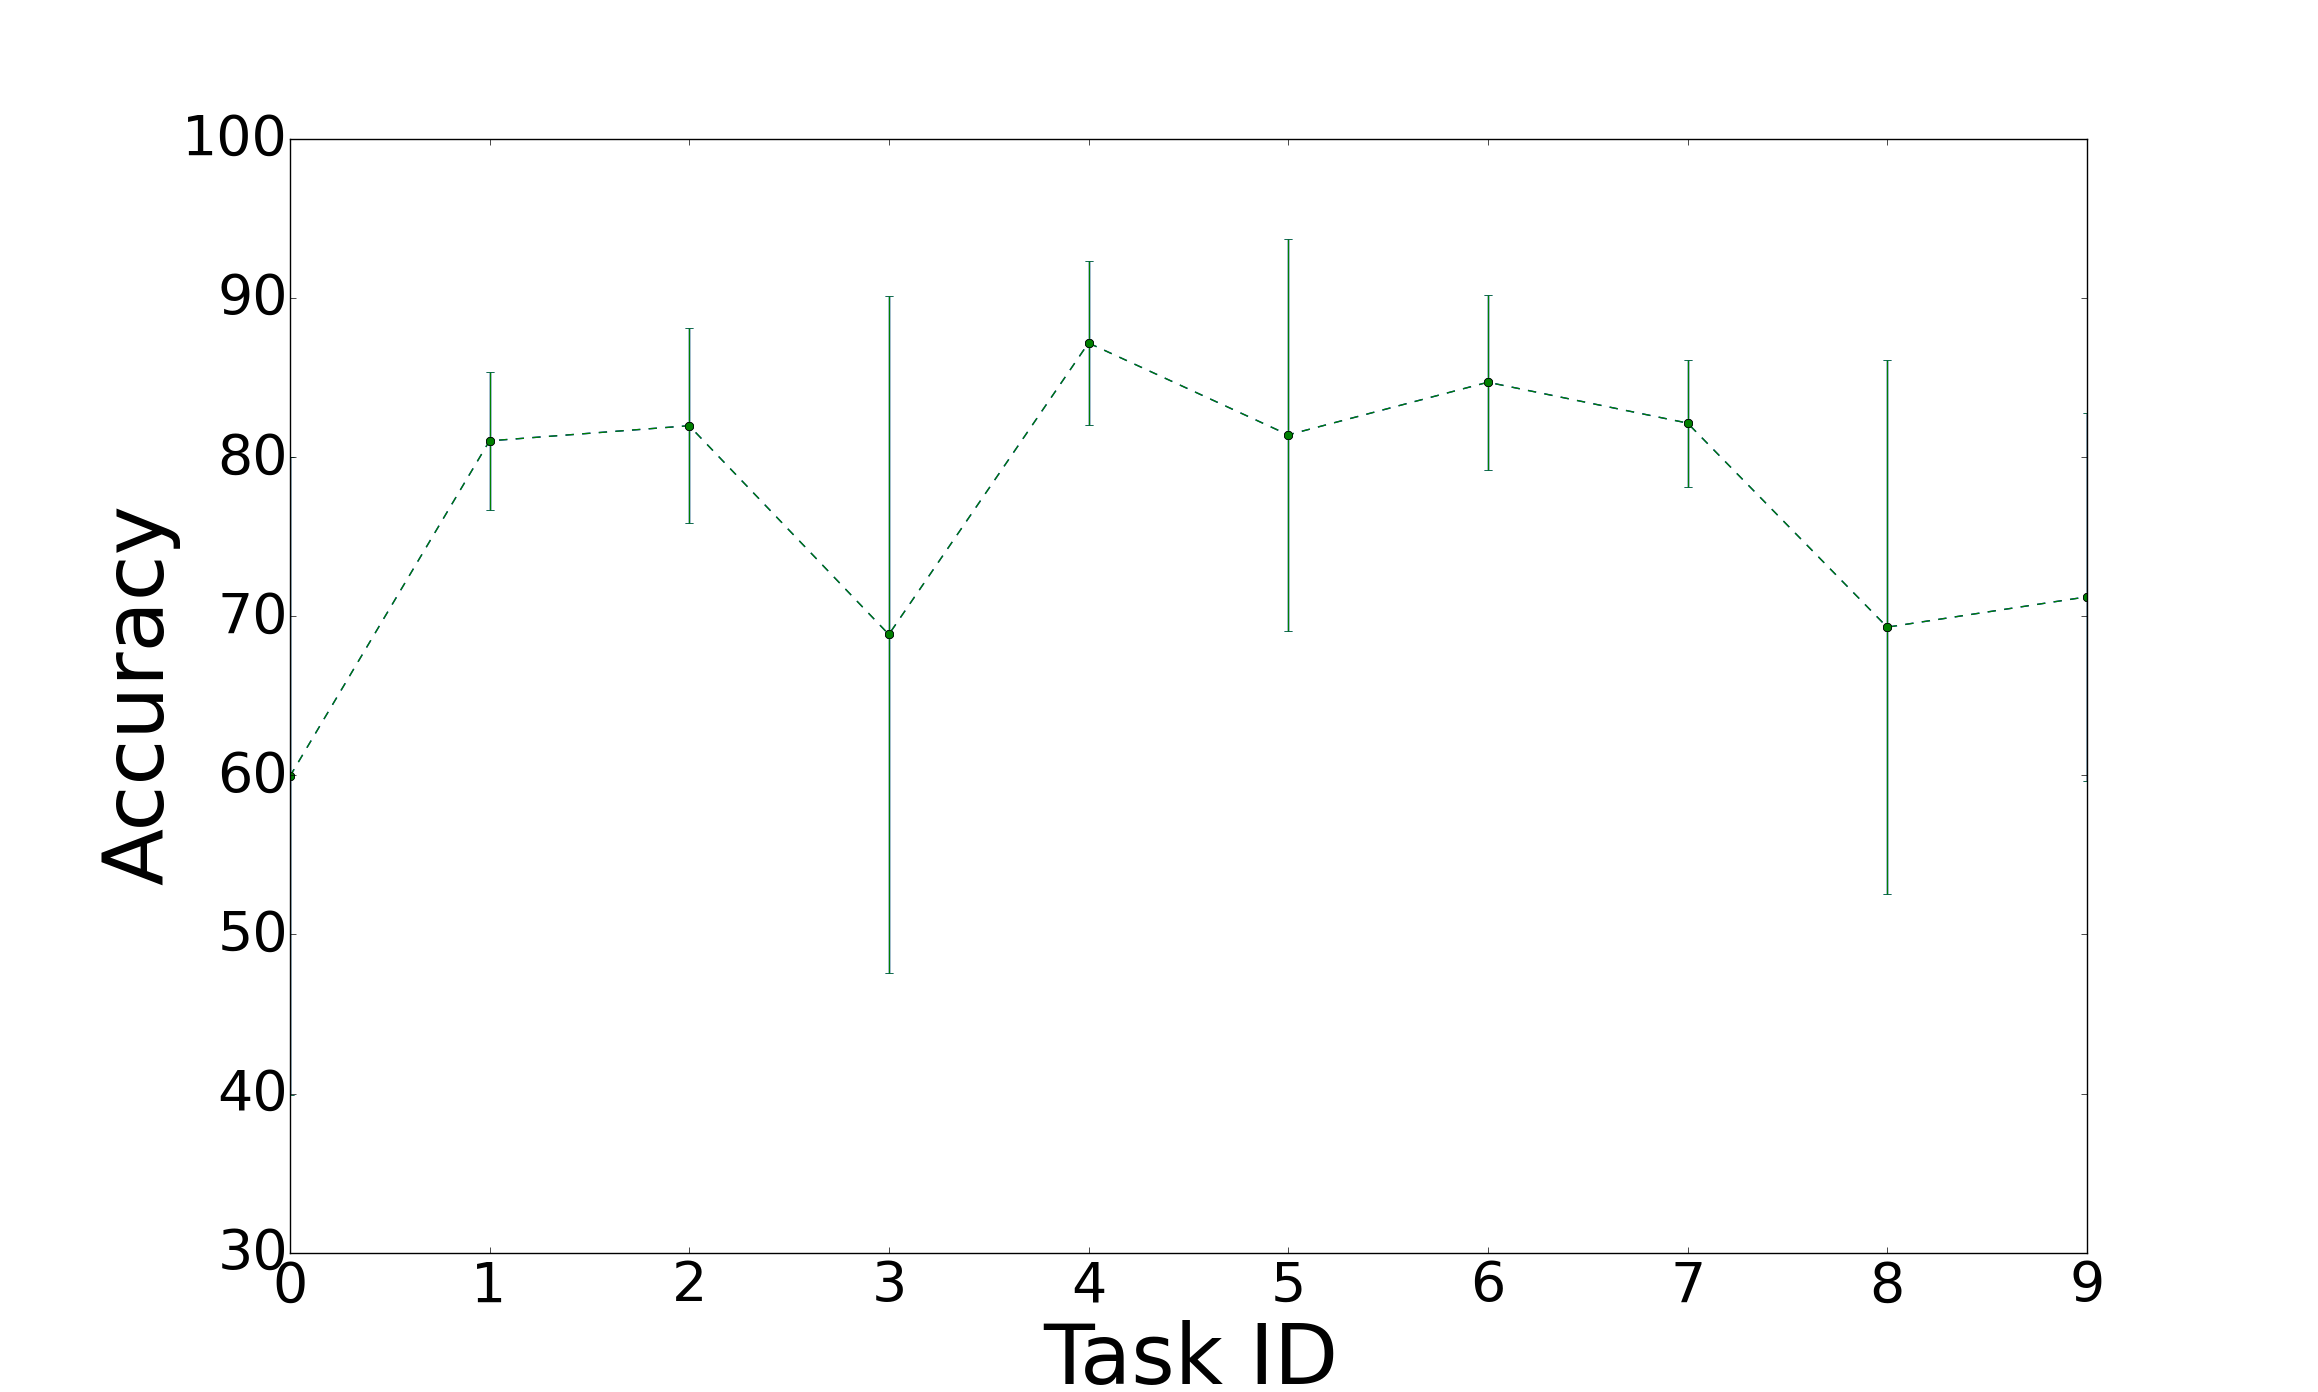
\includegraphics[width=\textwidth]{figures/plot_mlp}
        \caption{Active annotators for different total number}
    \end{subfigure}
    \begin{subfigure}[b]{0.45\textwidth}
        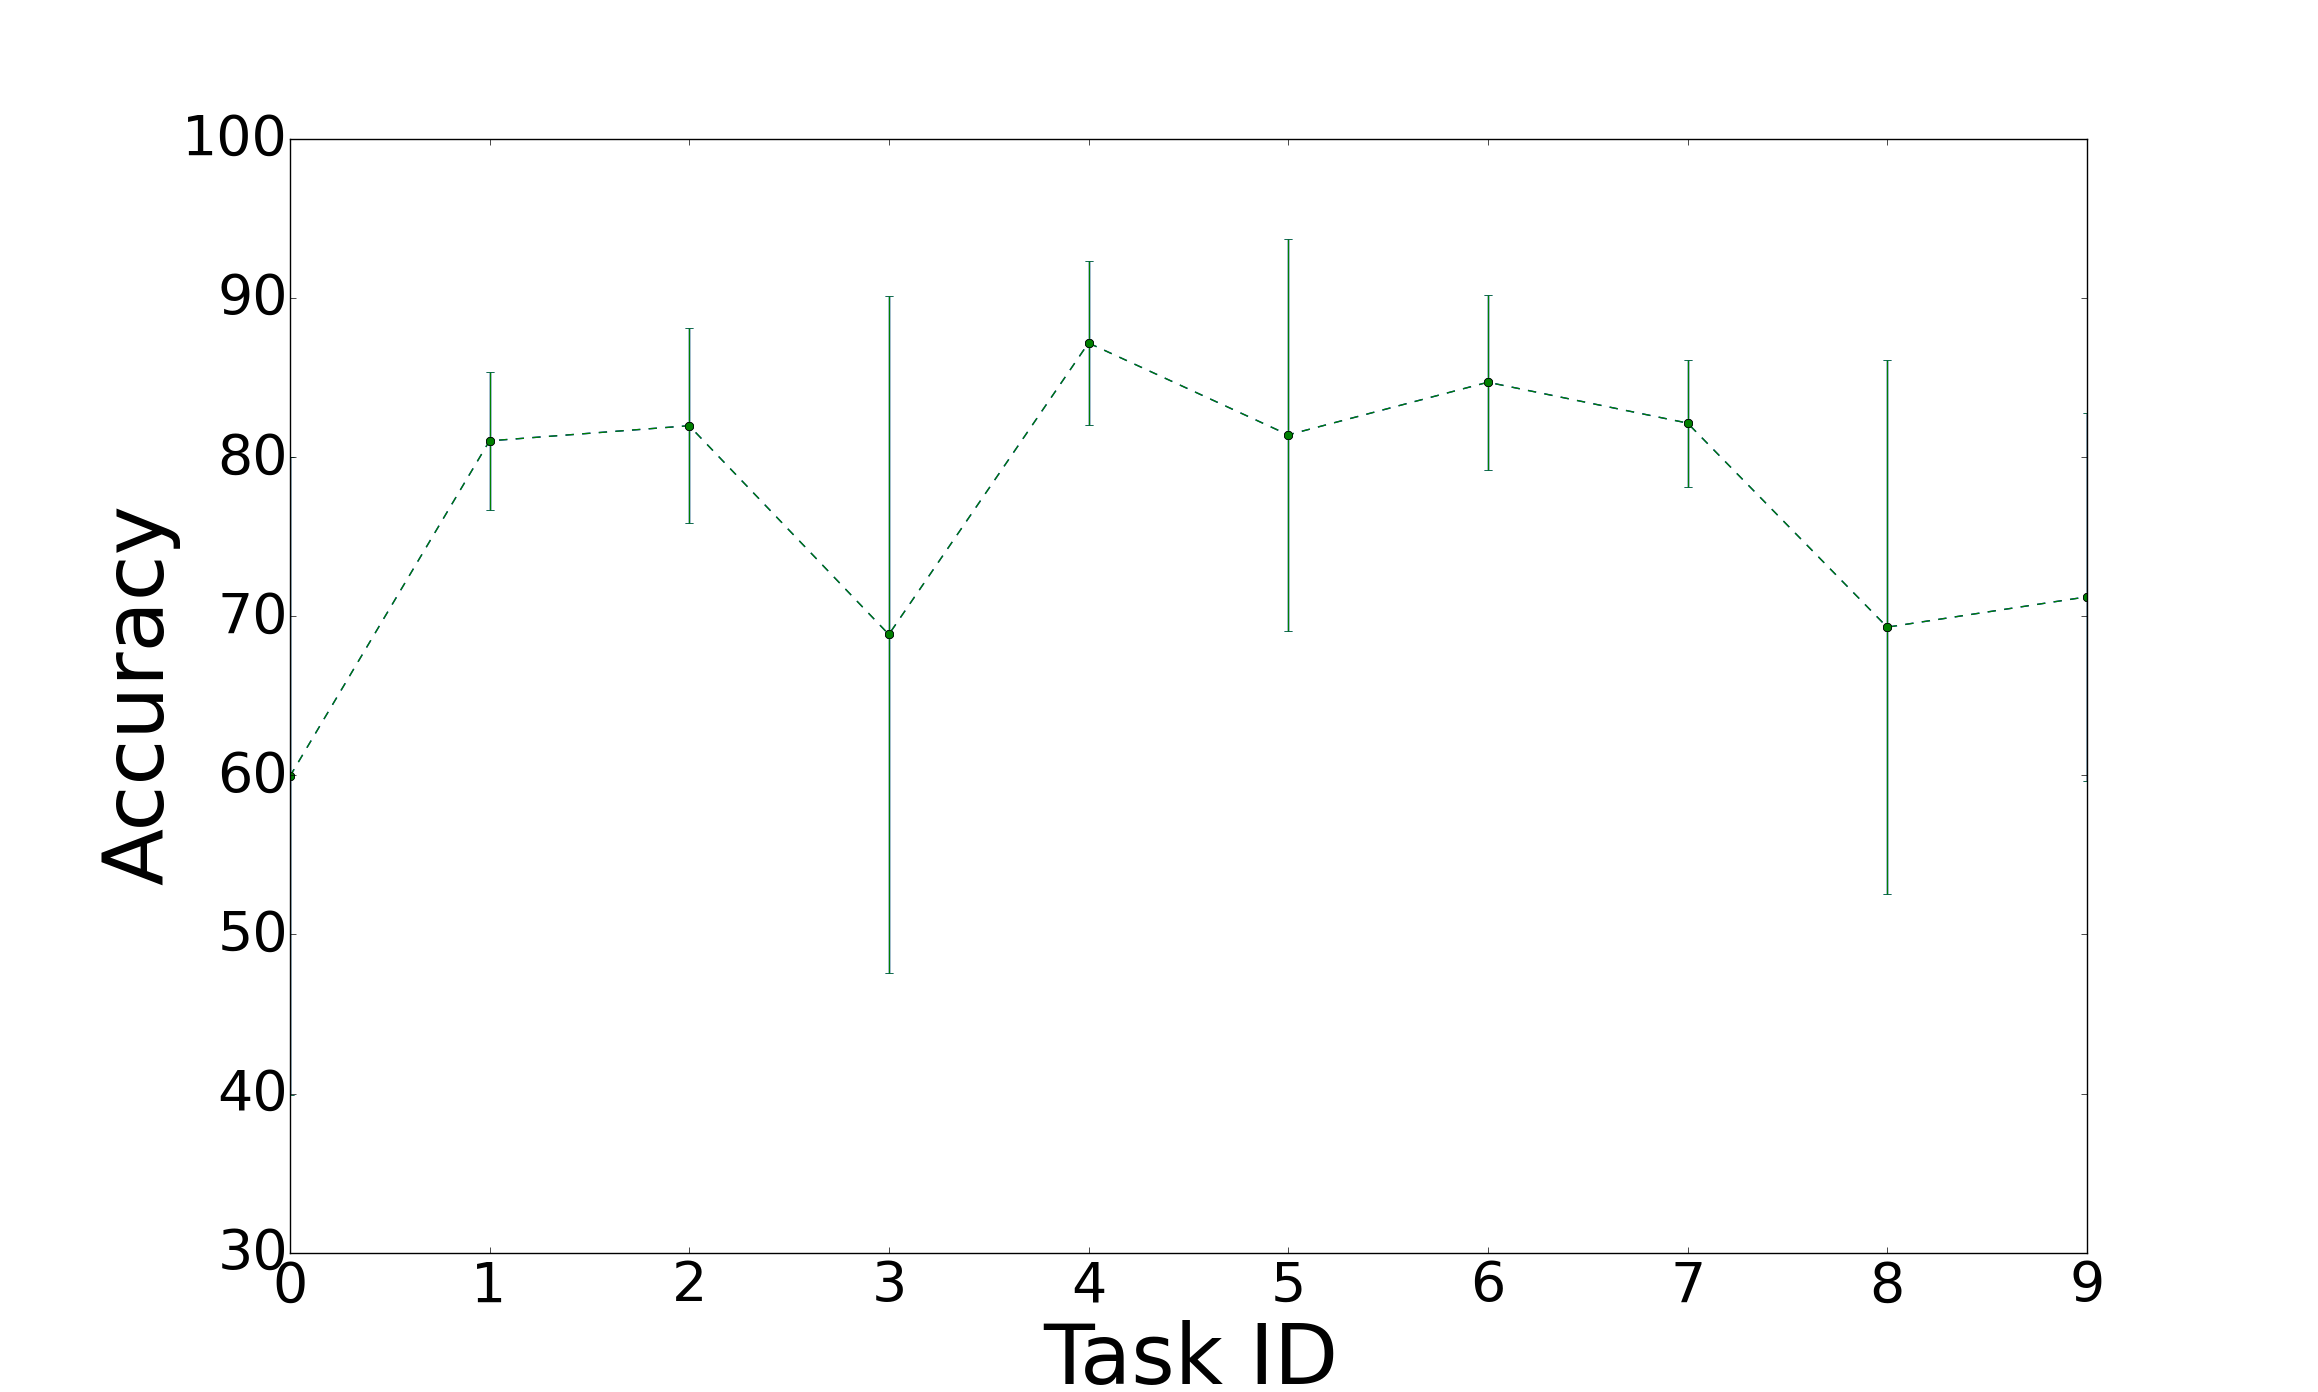
\includegraphics[width=\textwidth]{figures/plot_mlp}
        \caption{Accuracy for various initial number of annotators}
    \end{subfigure}
  \caption{Change of size of the annotator groups}
  \label{fig:subset}
\end{figure}




\section{Discussion}


\section{Conclusion}

\bibliographystyle{plain}
\bibliography{draft} 

\end{document}
